\documentclass[12pt, letterpaper, twoside]{book}
\raggedbottom
\usepackage{graphicx}
\graphicspath{ {images/} }
\usepackage[utf8]{inputenc}
\usepackage{fullpage}
\usepackage[paperheight=11in,paperwidth=8.5in,margin=0in]{geometry}
\usepackage{amsmath}
\usepackage{listings}
\date{3nd June 2021}
\begin{document}
\begin{titlepage}
	\begin{center}
       \vspace*{5cm}
       \bfseries\Large
    	Assignment 4\\
    	Of\\
    	Modelling \& Simulation Lab (CS1052)\\
        \vskip1cm
        Masters of Technology in Computer Science And Engineering\\
        \vskip1cm
        submitted by\\
    	Arghya Bandyopadhyay\\
    	RollNo. 20CS4103\\
    	\vskip1cm
    	submitted to\\
    	Dr Nanda Dulal Jana\\
    	Assistant Professor\\
    	Dept. of CSE\\
    	\vskip1cm
    	
\includegraphics[width=4cm]{NITDGP}\\
    	National Institute of Technology, Durgapur\\
    \end{center}
\end{titlepage}
\begin{center}
\textbf{\\Problem 1}
\end{center}
\begin{flushleft}
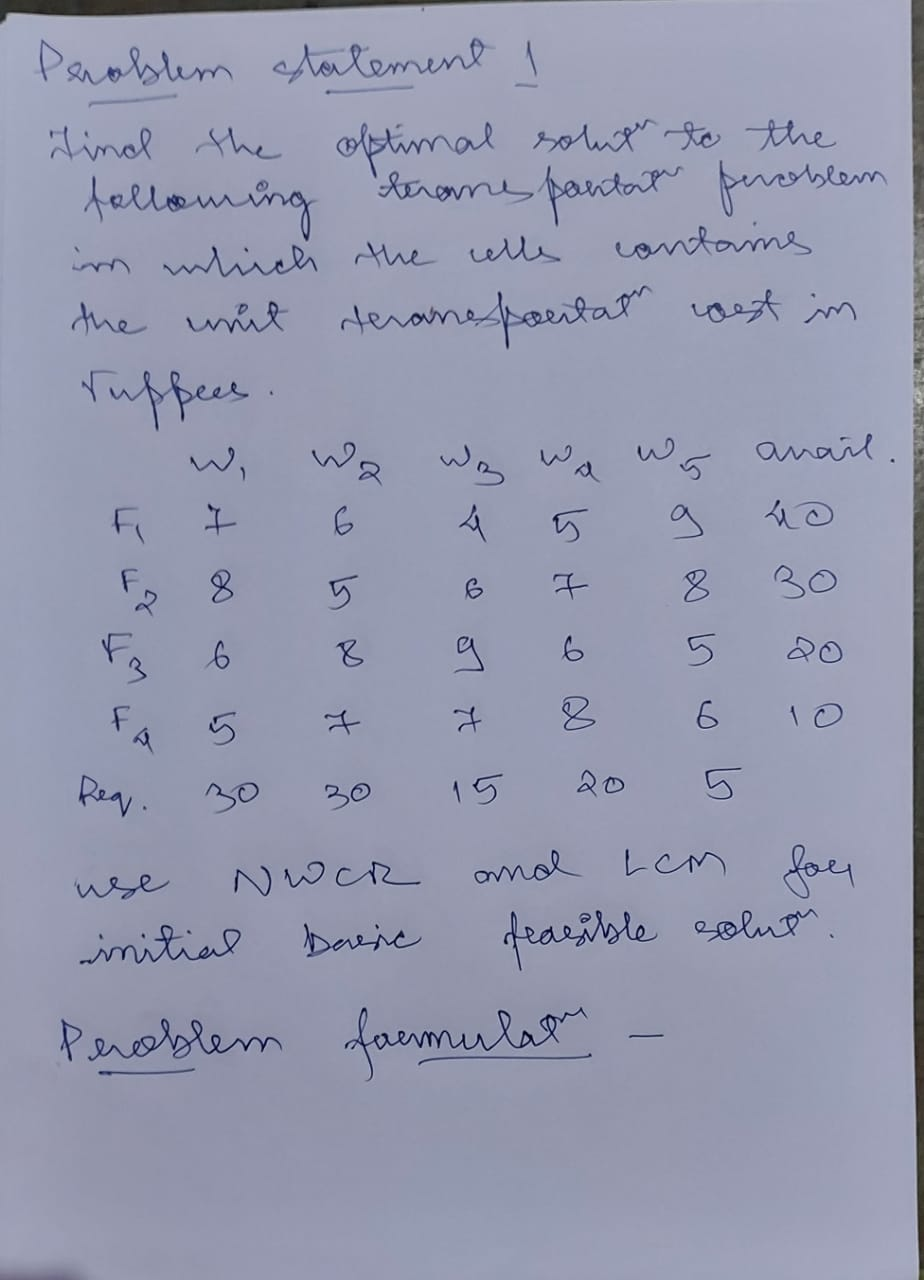
\includegraphics[width=\paperwidth, height=10in]{Page1}
\end{flushleft}
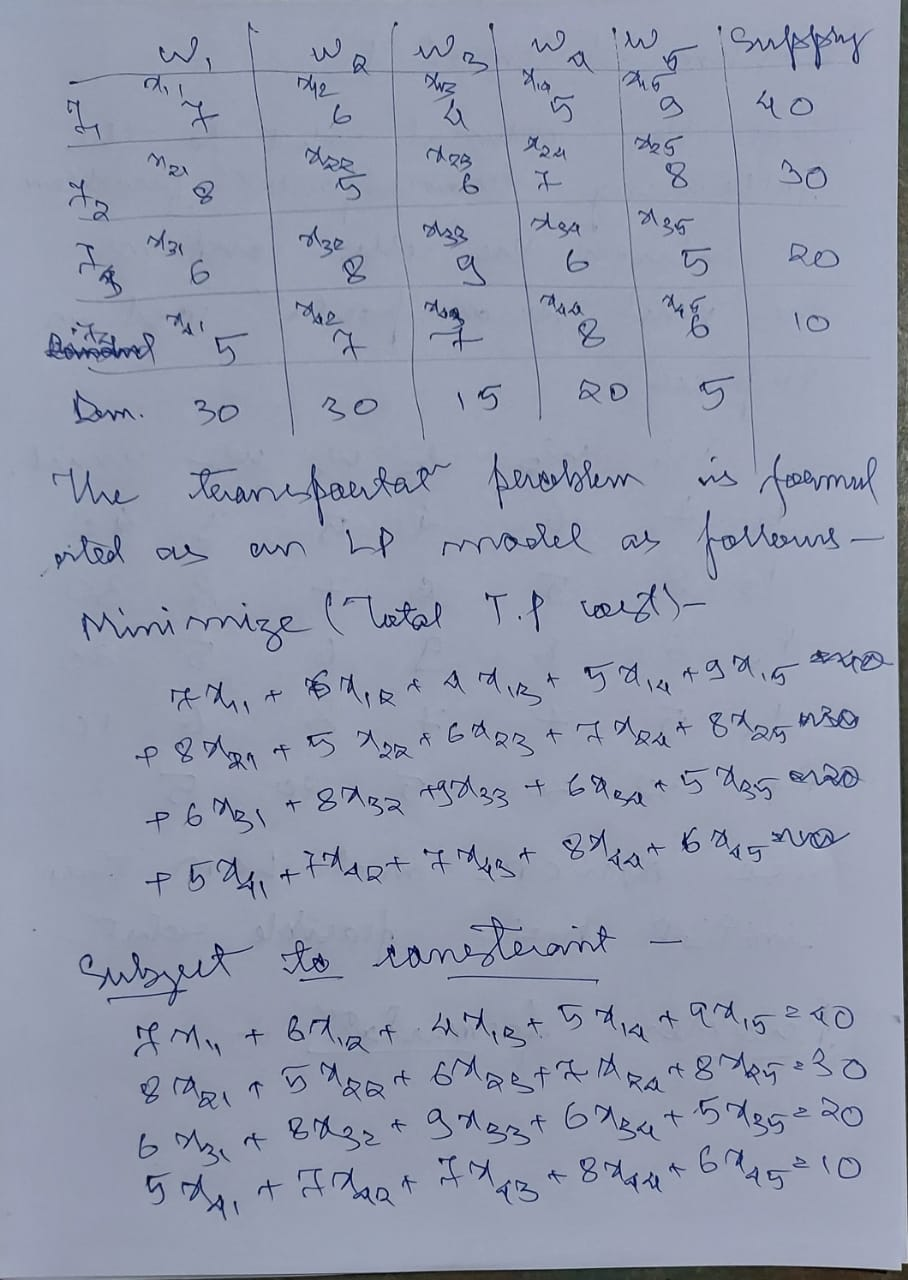
\includegraphics[width=\paperwidth, height=\paperheight]{Page2}
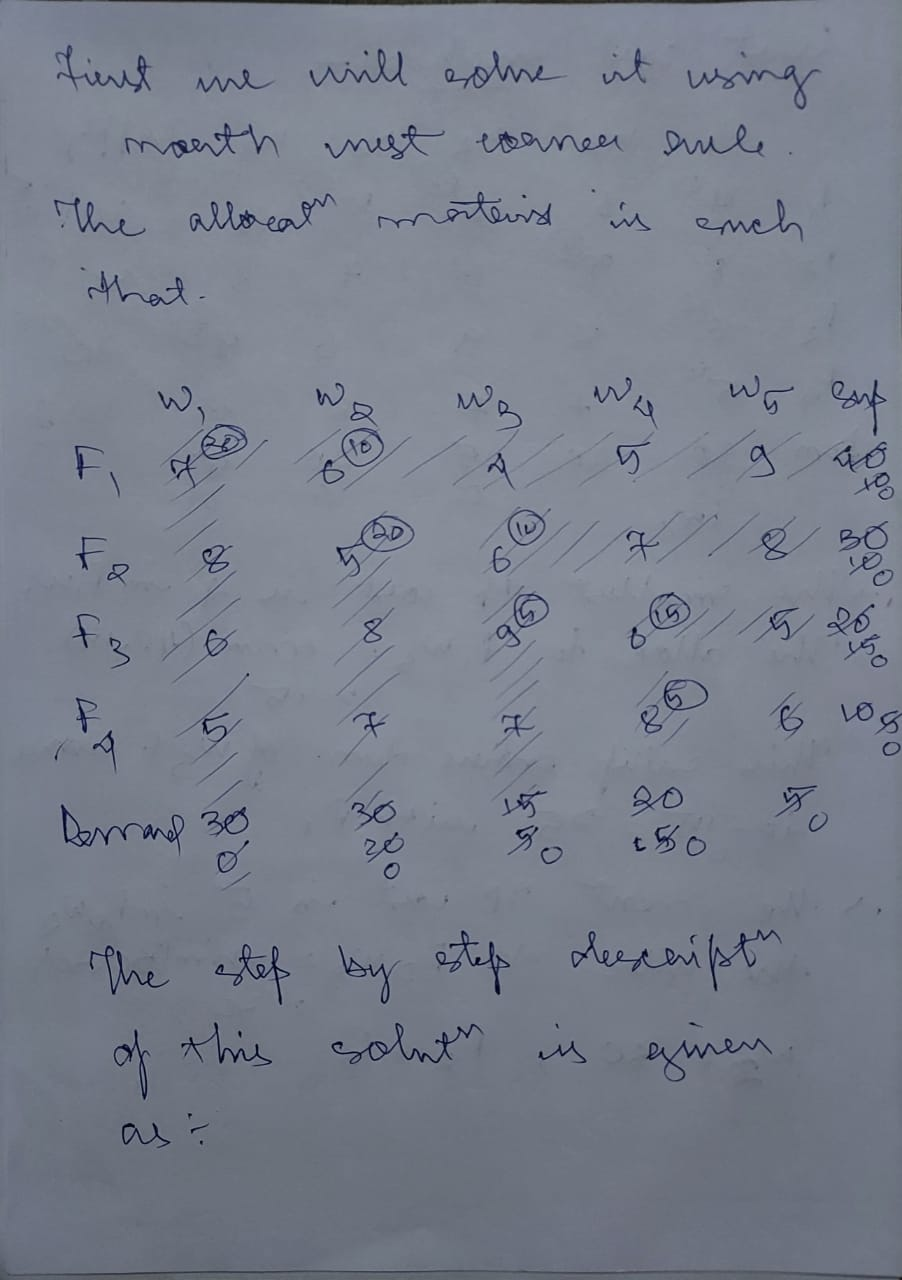
\includegraphics[width=\paperwidth, height=\paperheight]{Page3}
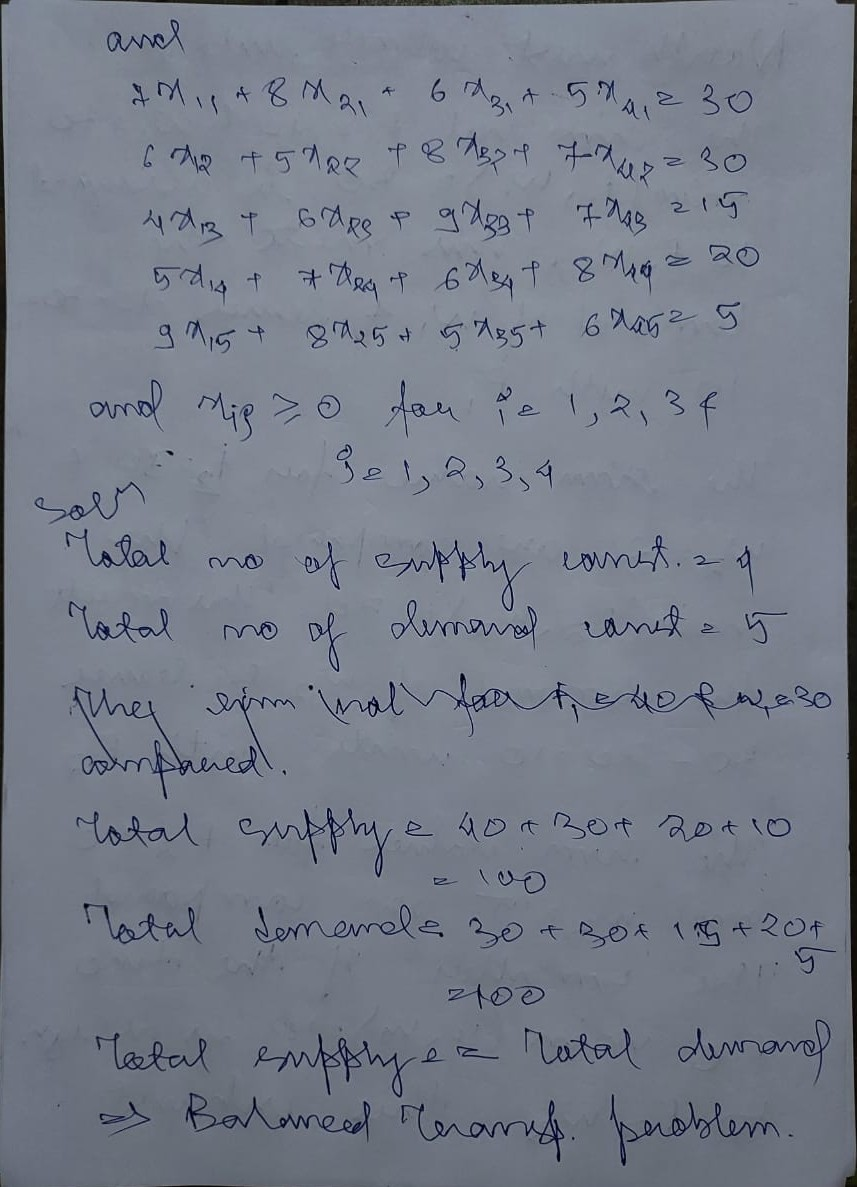
\includegraphics[width=\paperwidth, height=\paperheight]{Page4}
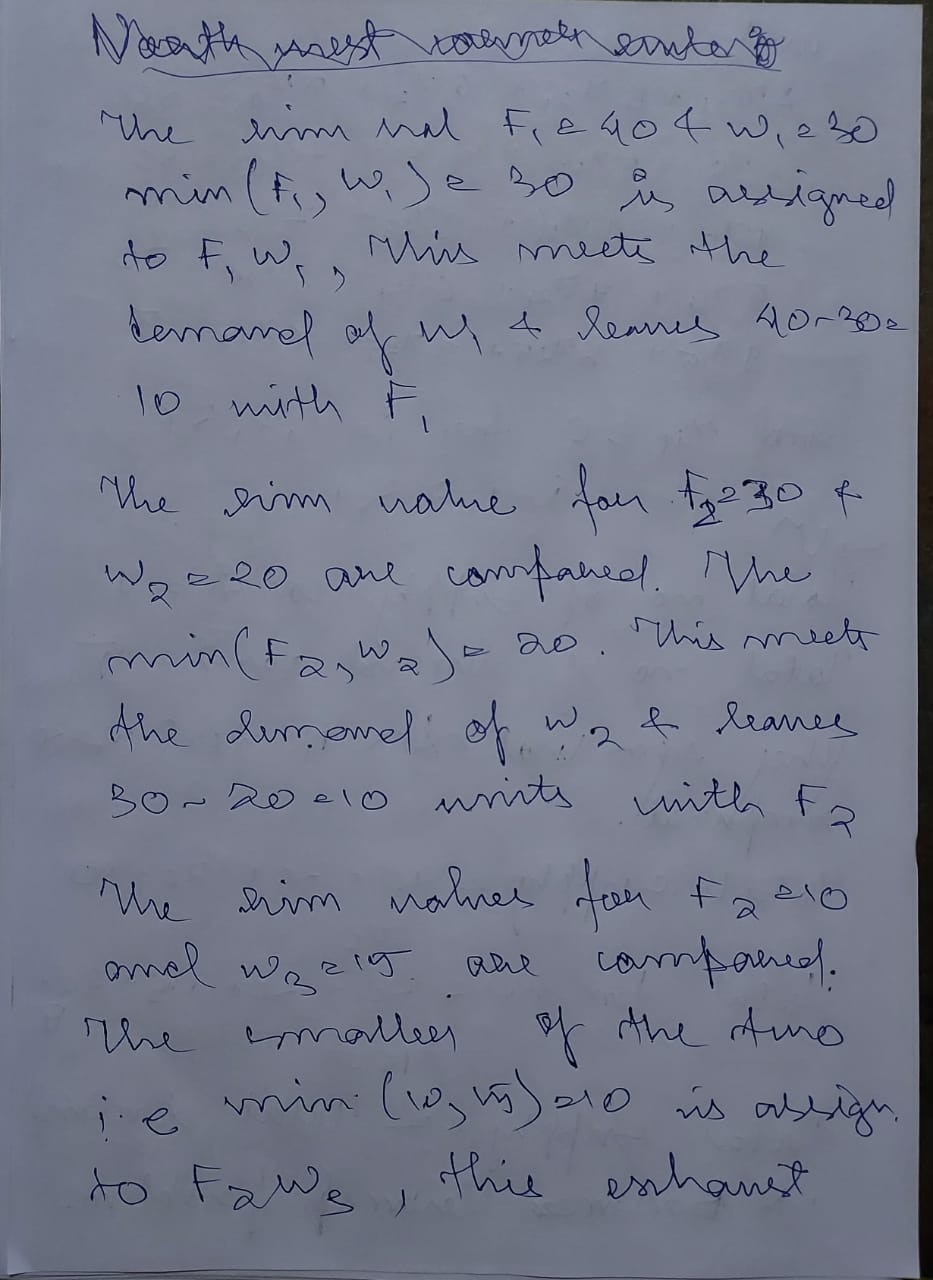
\includegraphics[width=\paperwidth, height=\paperheight]{Page5}
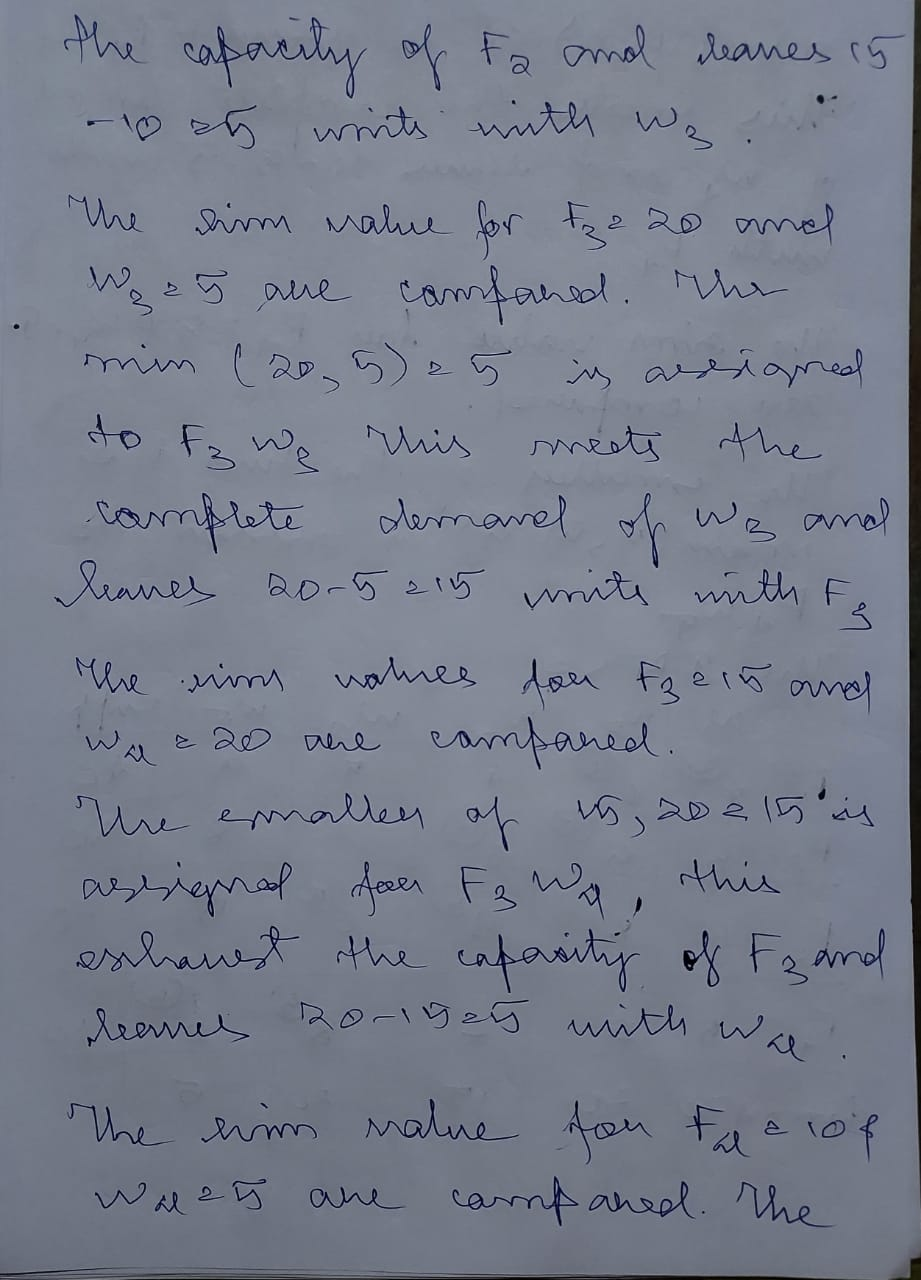
\includegraphics[width=\paperwidth, height=\paperheight]{Page6}
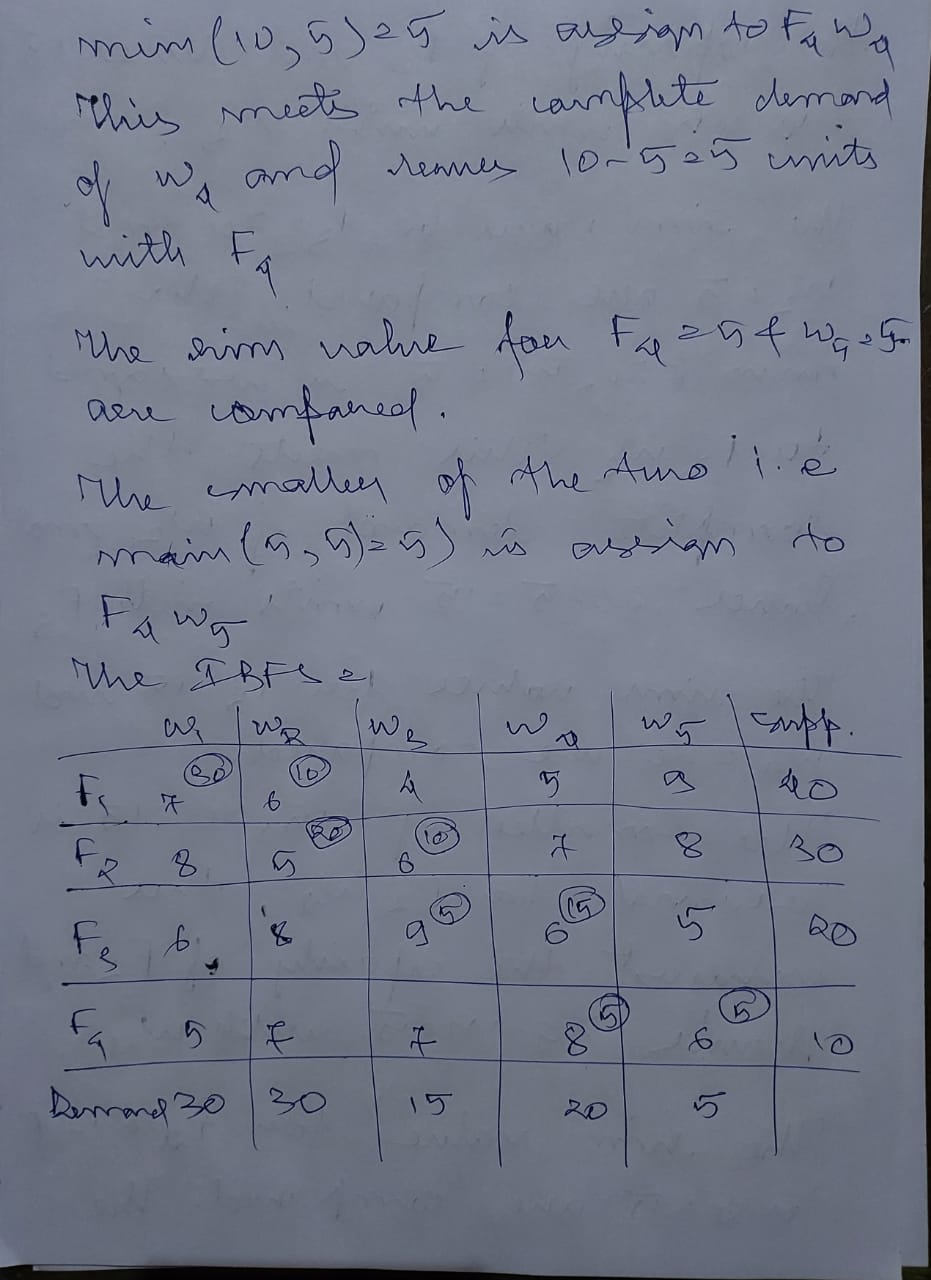
\includegraphics[width=\paperwidth, height=\paperheight]{Page7}
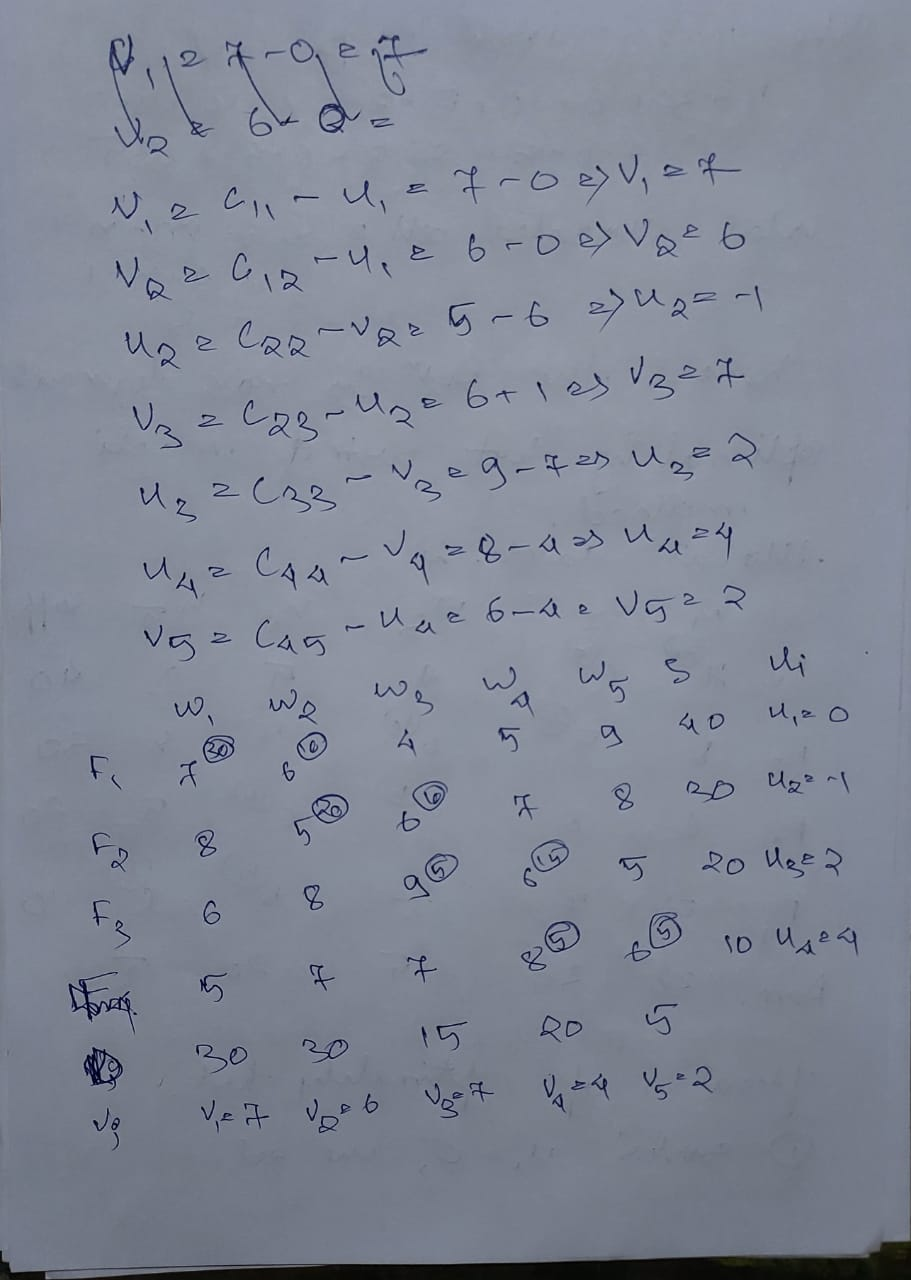
\includegraphics[width=\paperwidth, height=\paperheight]{Page8}
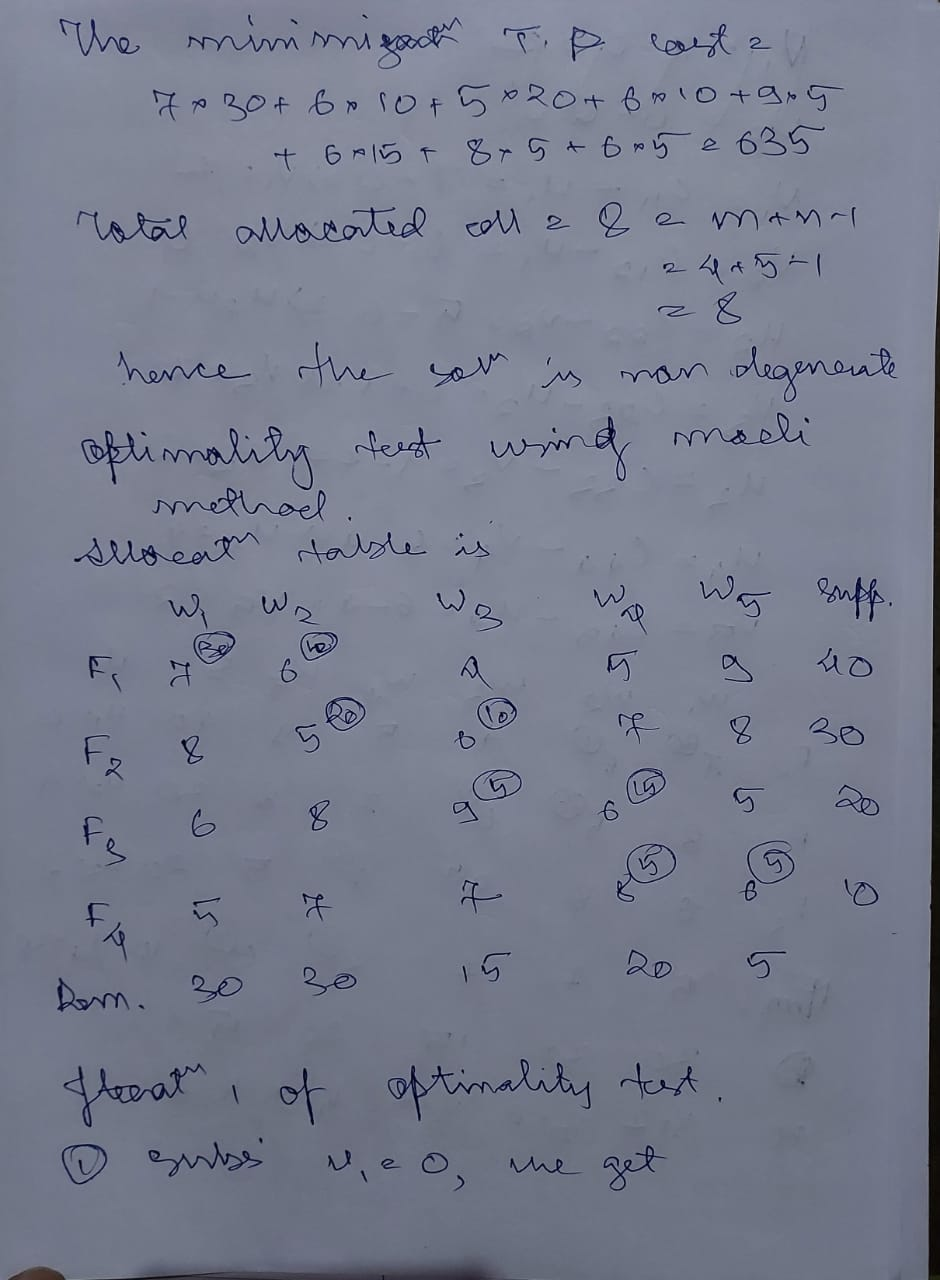
\includegraphics[width=\paperwidth, height=\paperheight]{Page9}
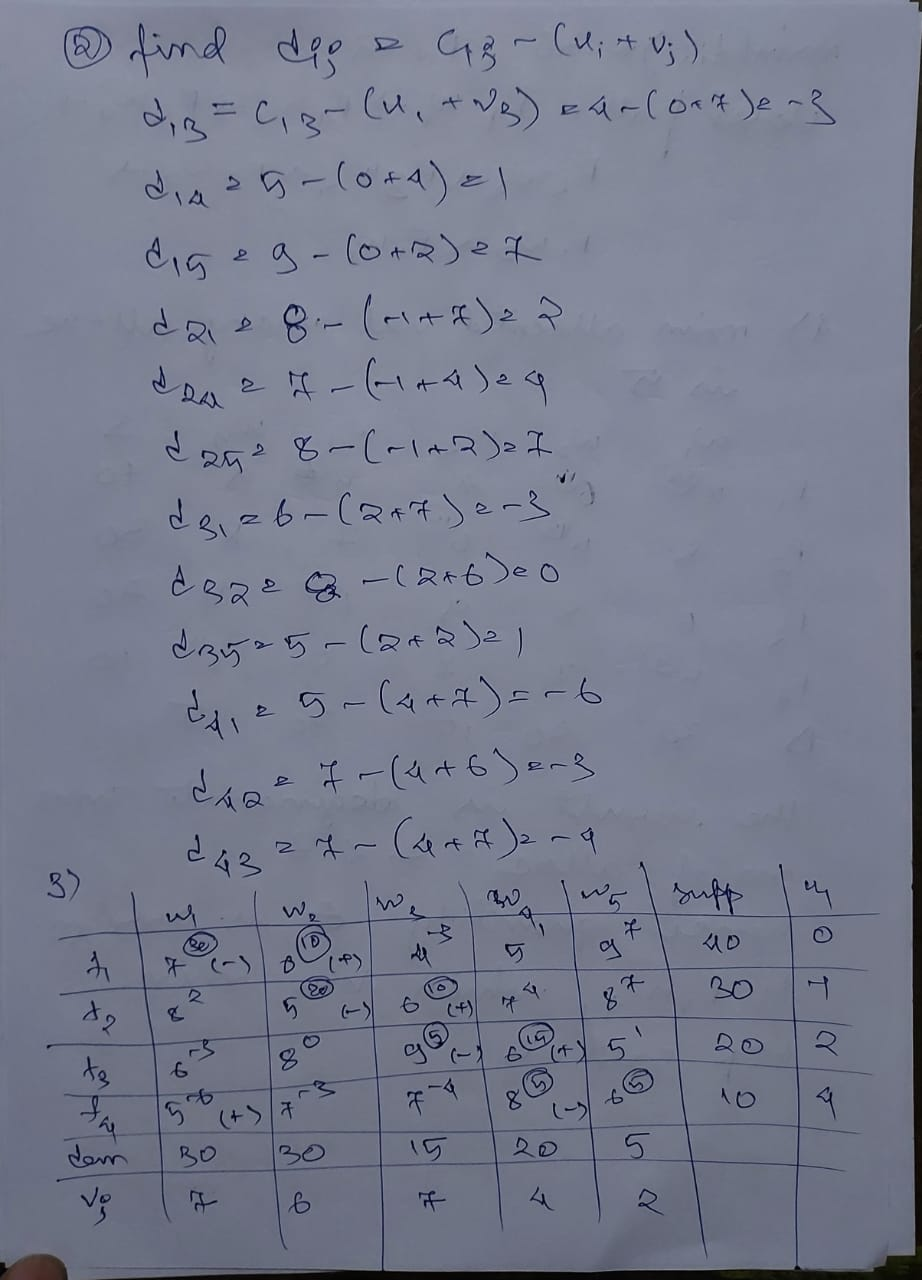
\includegraphics[width=\paperwidth, height=\paperheight]{Page10}
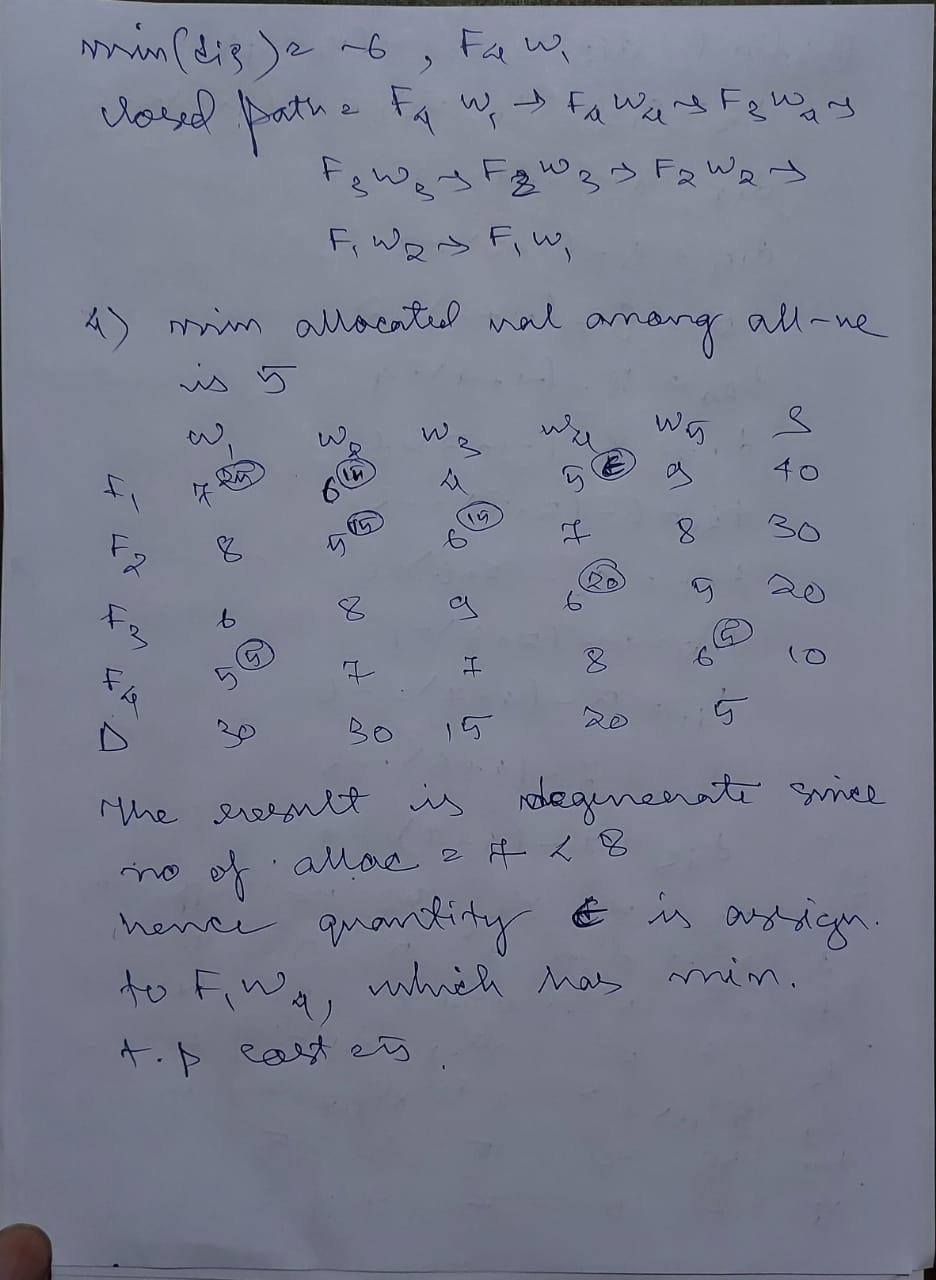
\includegraphics[width=\paperwidth, height=\paperheight]{Page11}
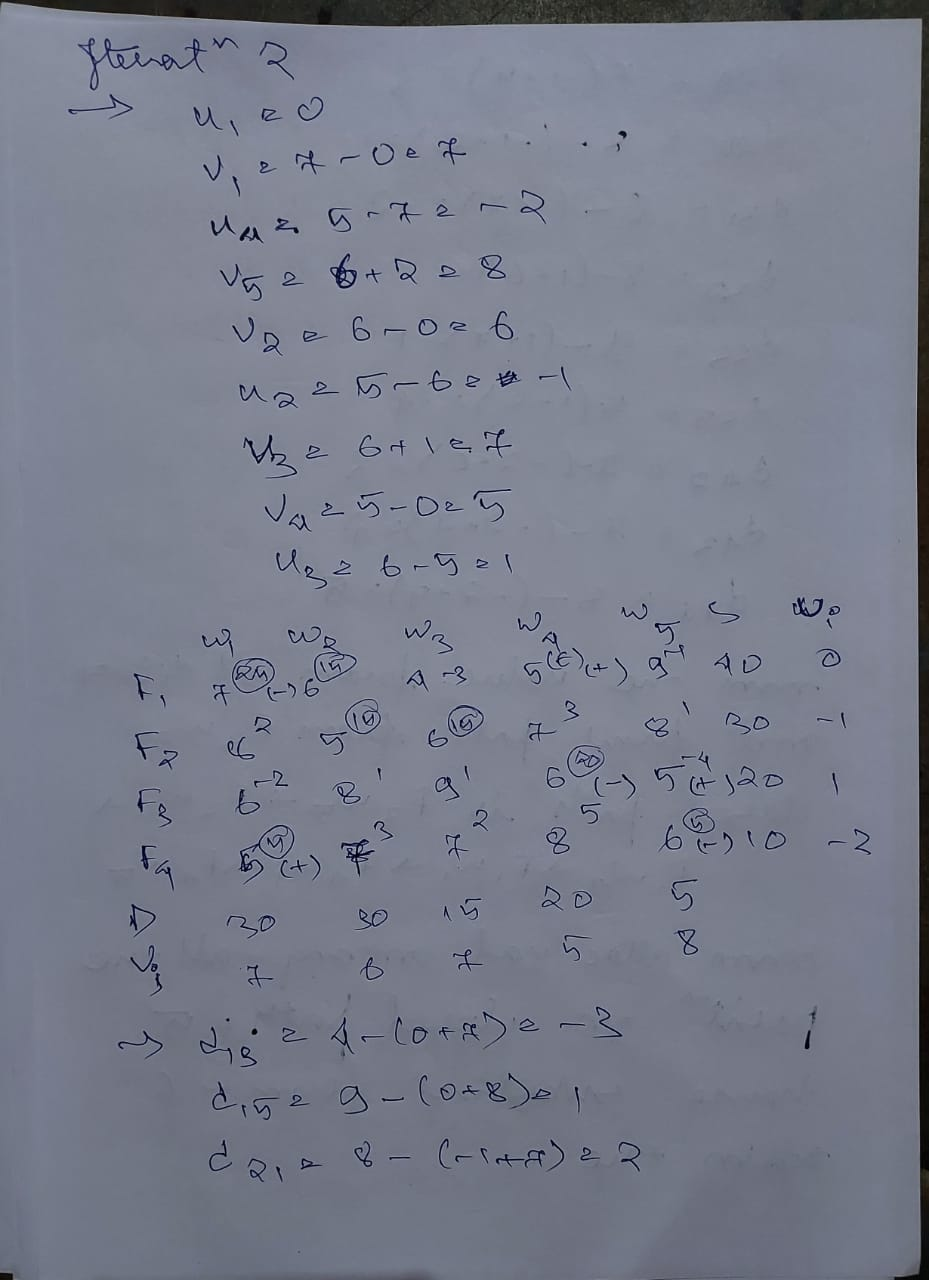
\includegraphics[width=\paperwidth, height=\paperheight]{Page12}
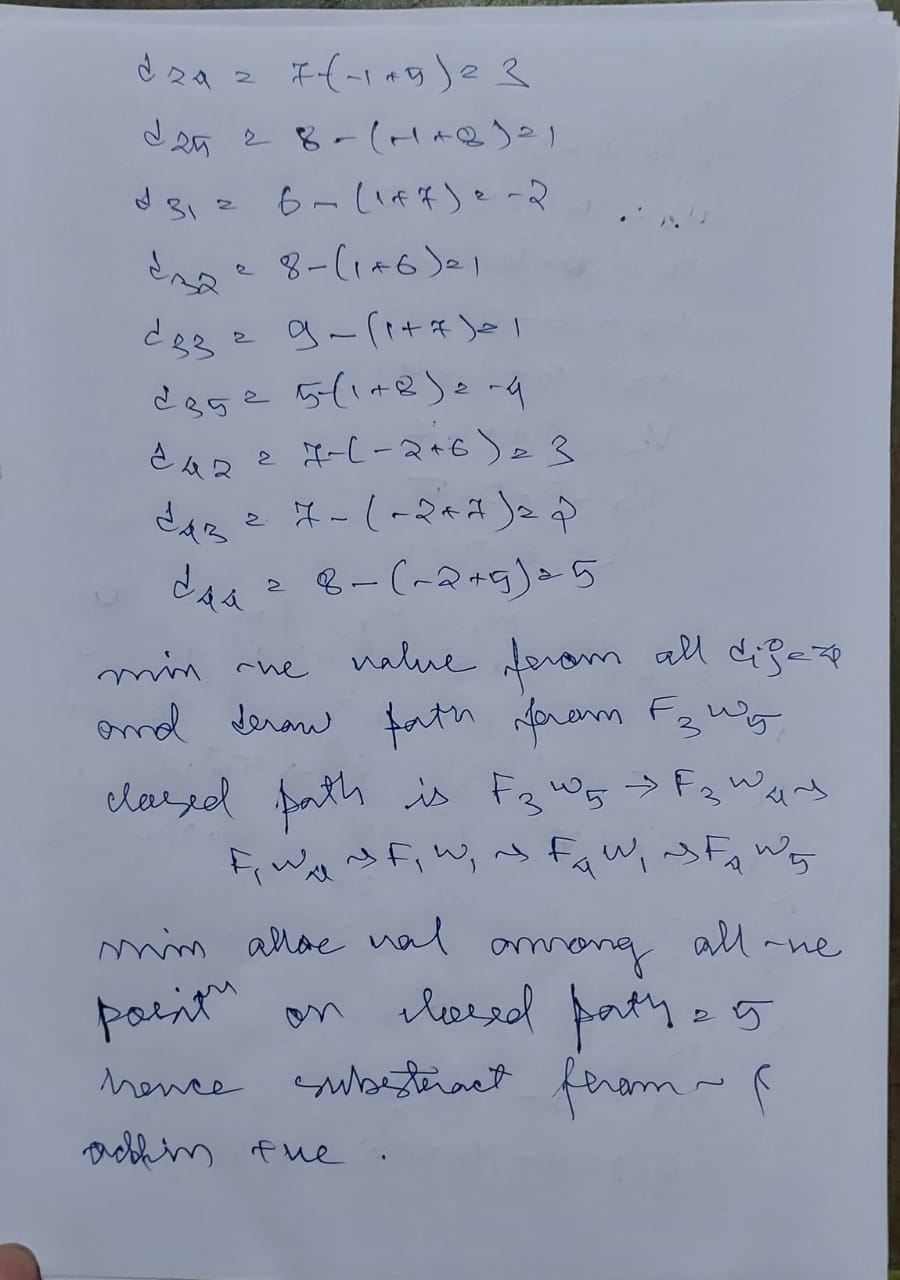
\includegraphics[width=\paperwidth, height=\paperheight]{Page13}
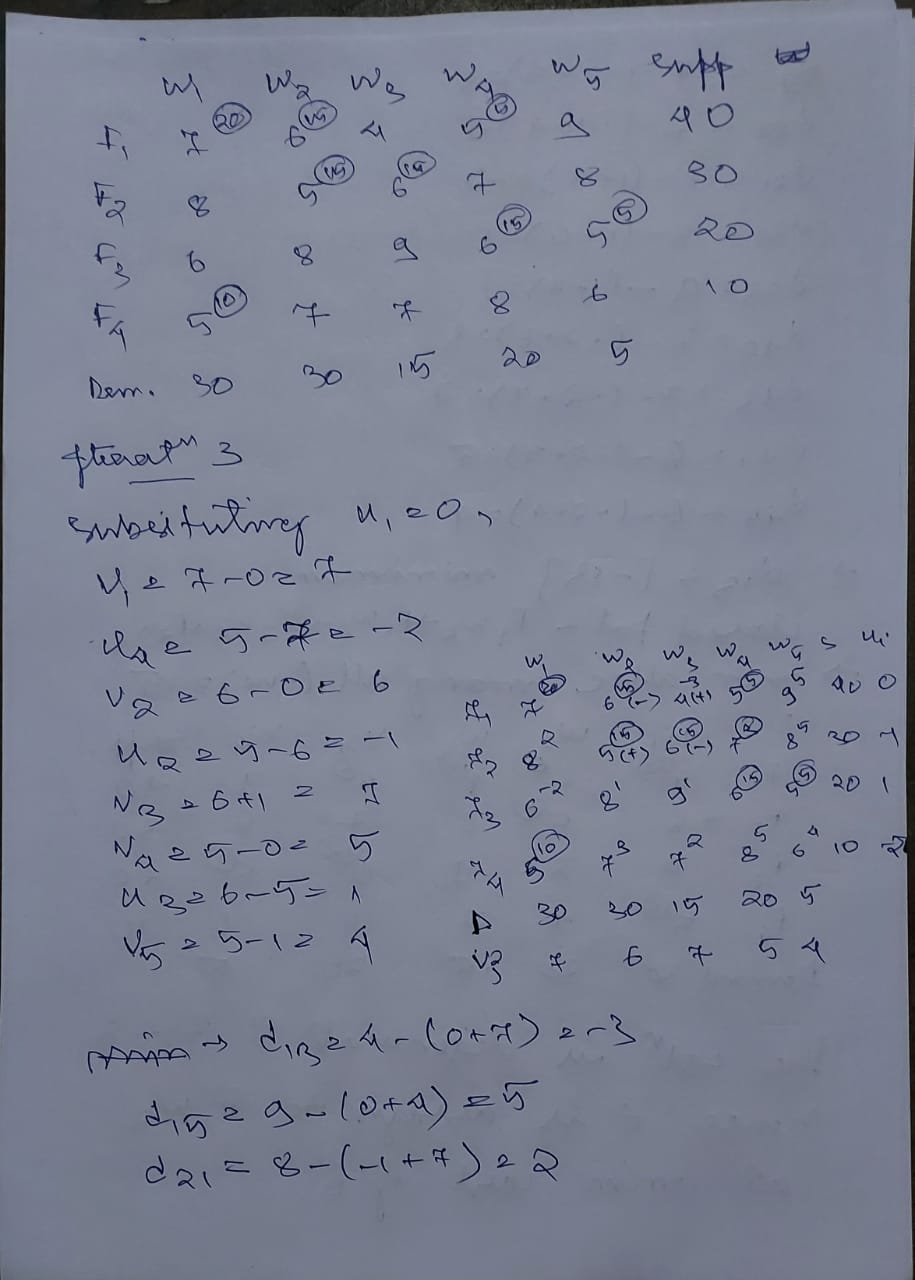
\includegraphics[width=\paperwidth, height=\paperheight]{Page14}
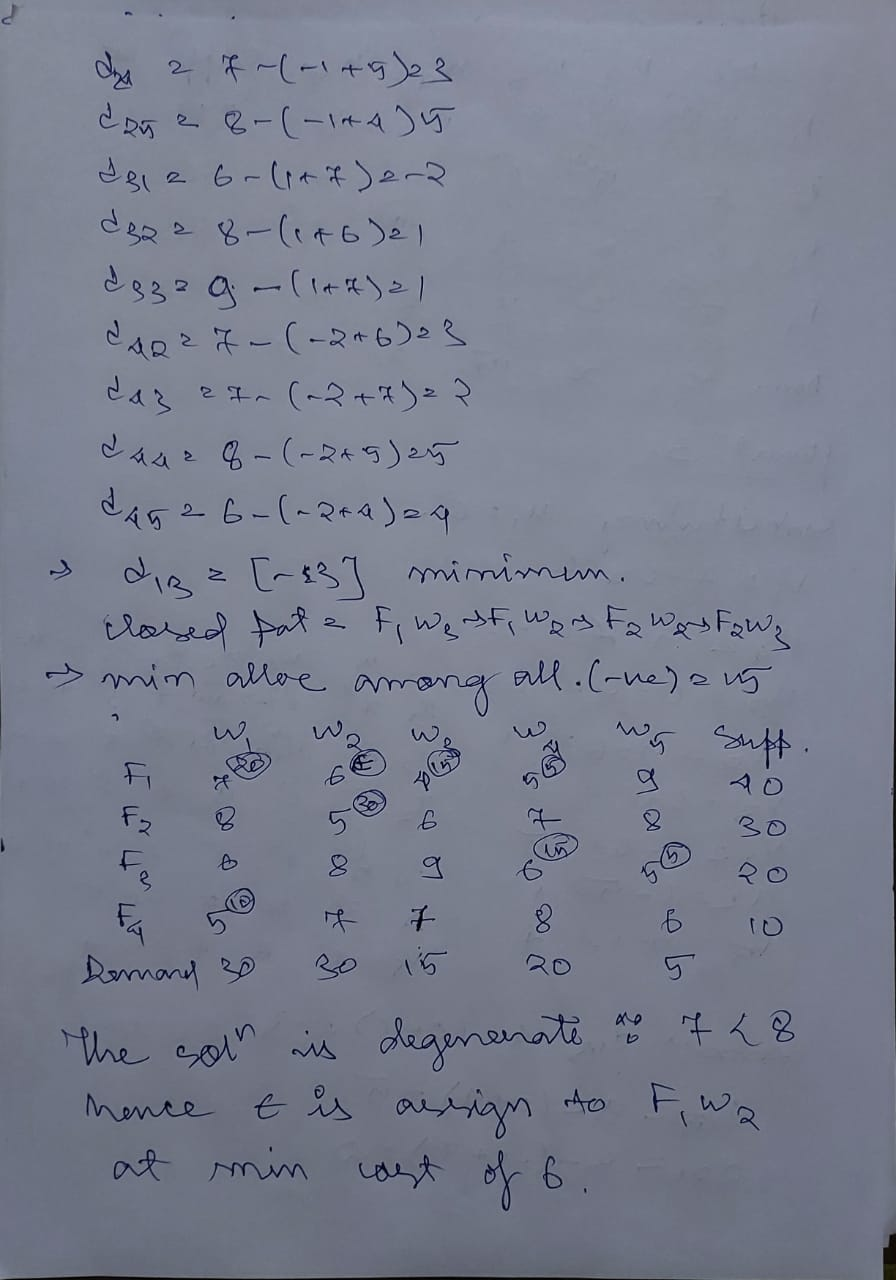
\includegraphics[width=\paperwidth, height=\paperheight]{Page15}
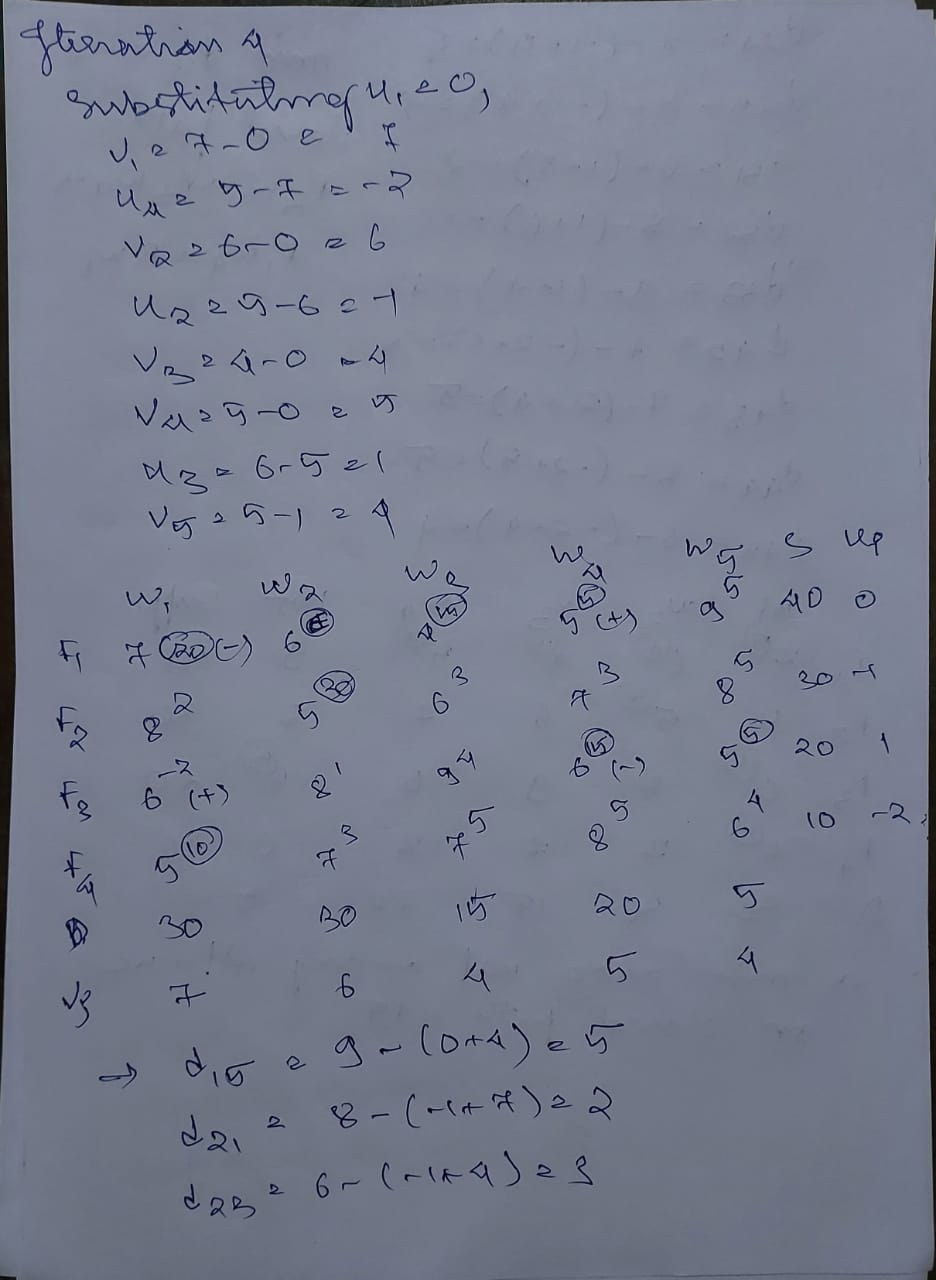
\includegraphics[width=\paperwidth, height=\paperheight]{Page16}
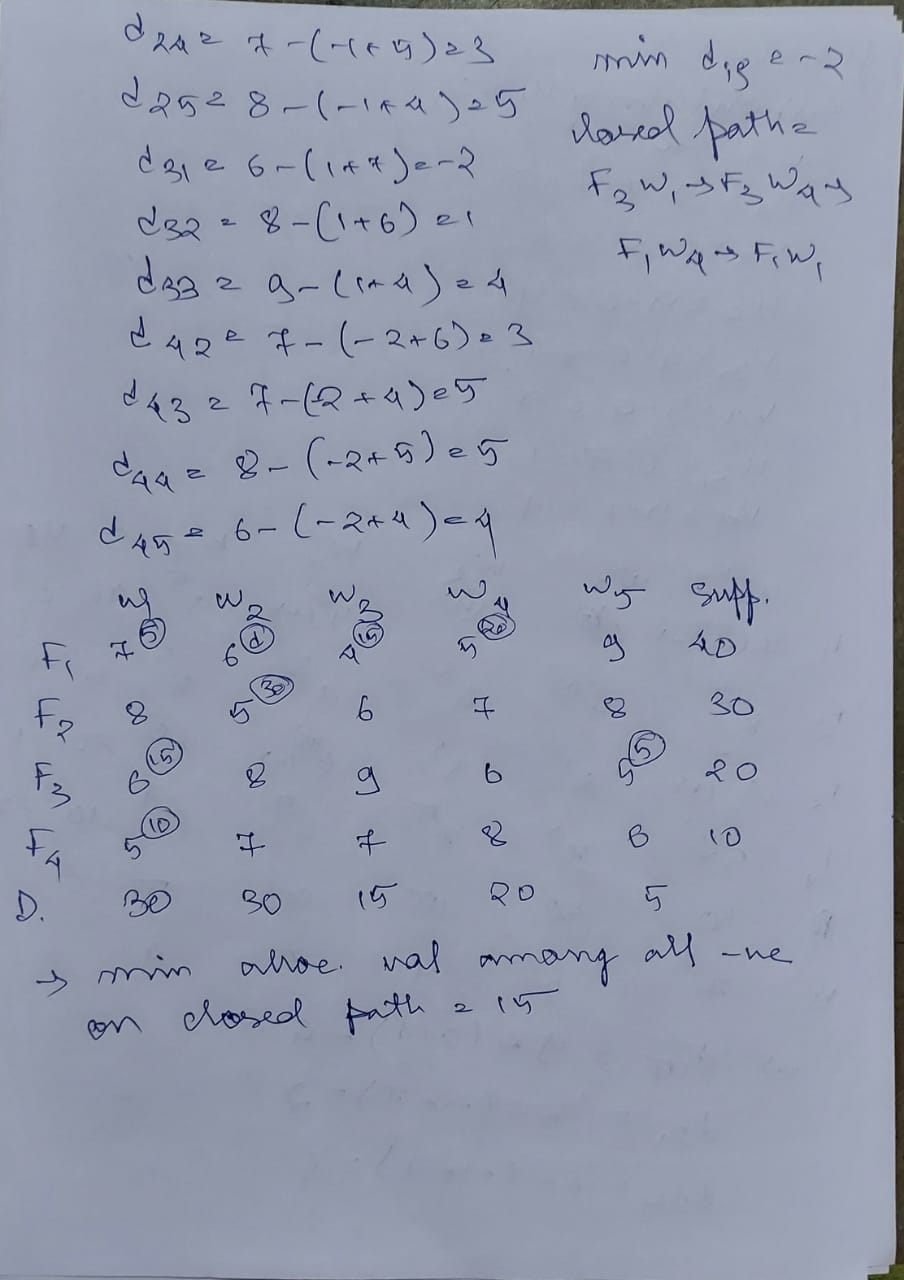
\includegraphics[width=\paperwidth, height=\paperheight]{Page17}
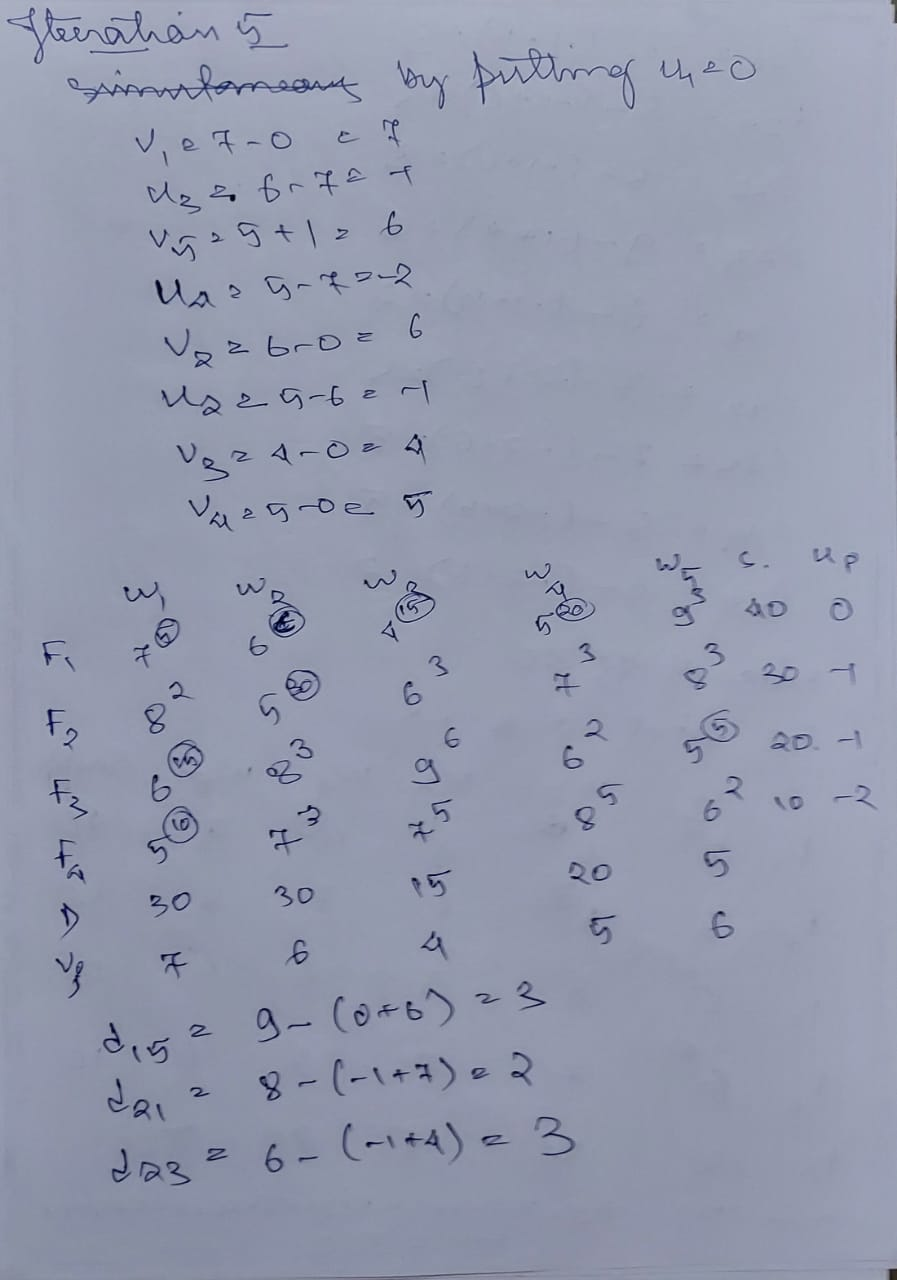
\includegraphics[width=\paperwidth, height=\paperheight]{Page18}
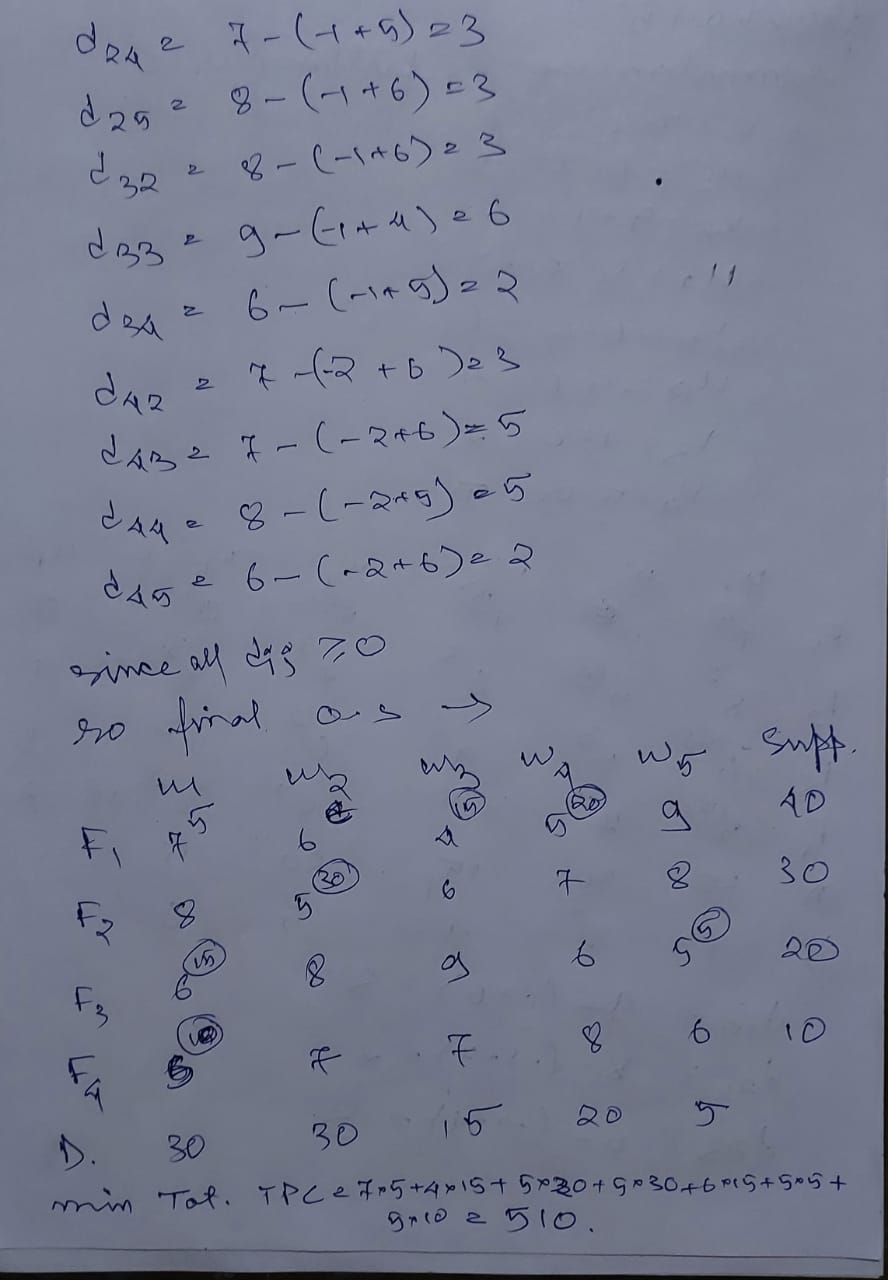
\includegraphics[width=\paperwidth, height=\paperheight]{Page19}
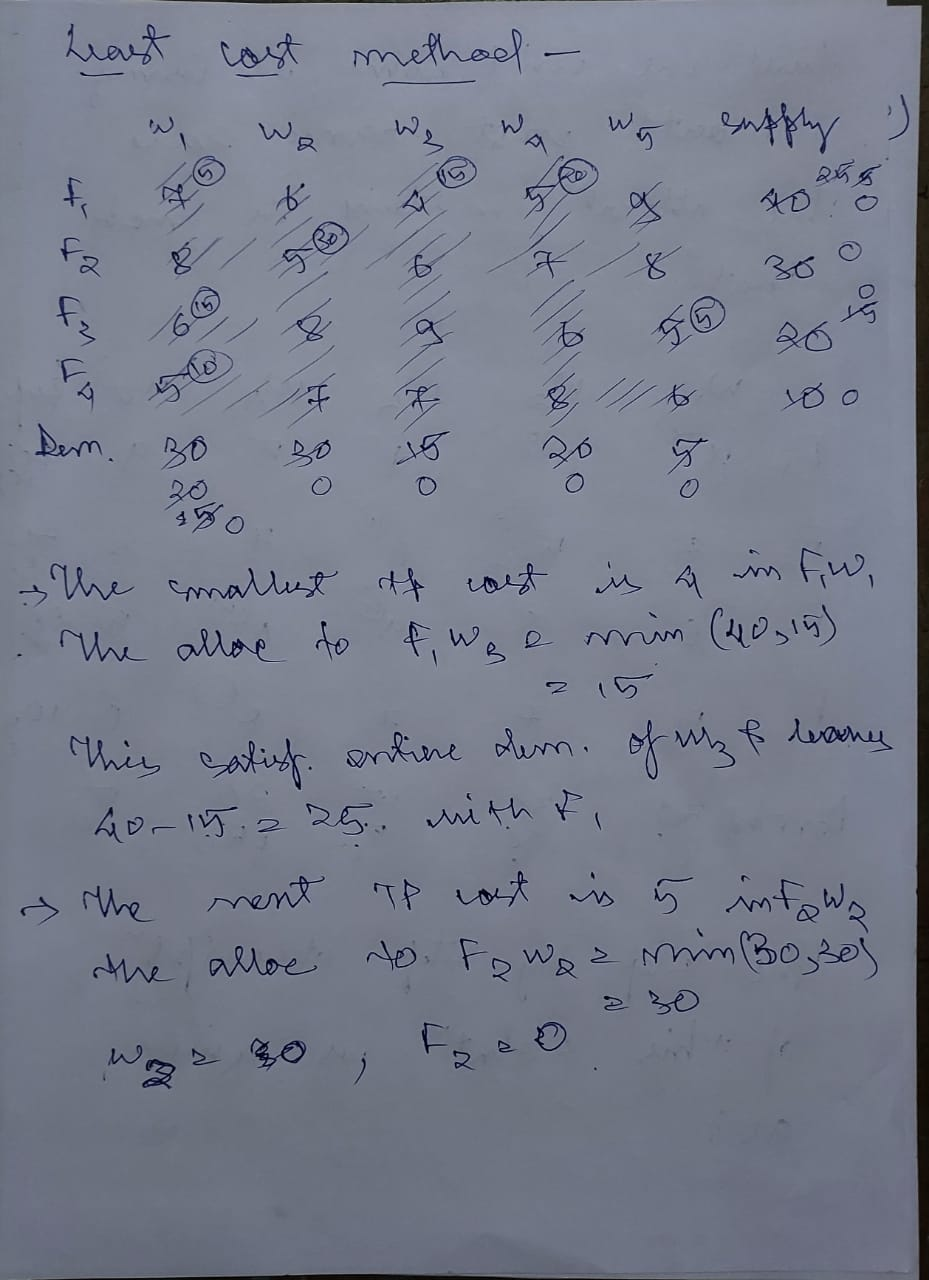
\includegraphics[width=\paperwidth, height=\paperheight]{Page20}
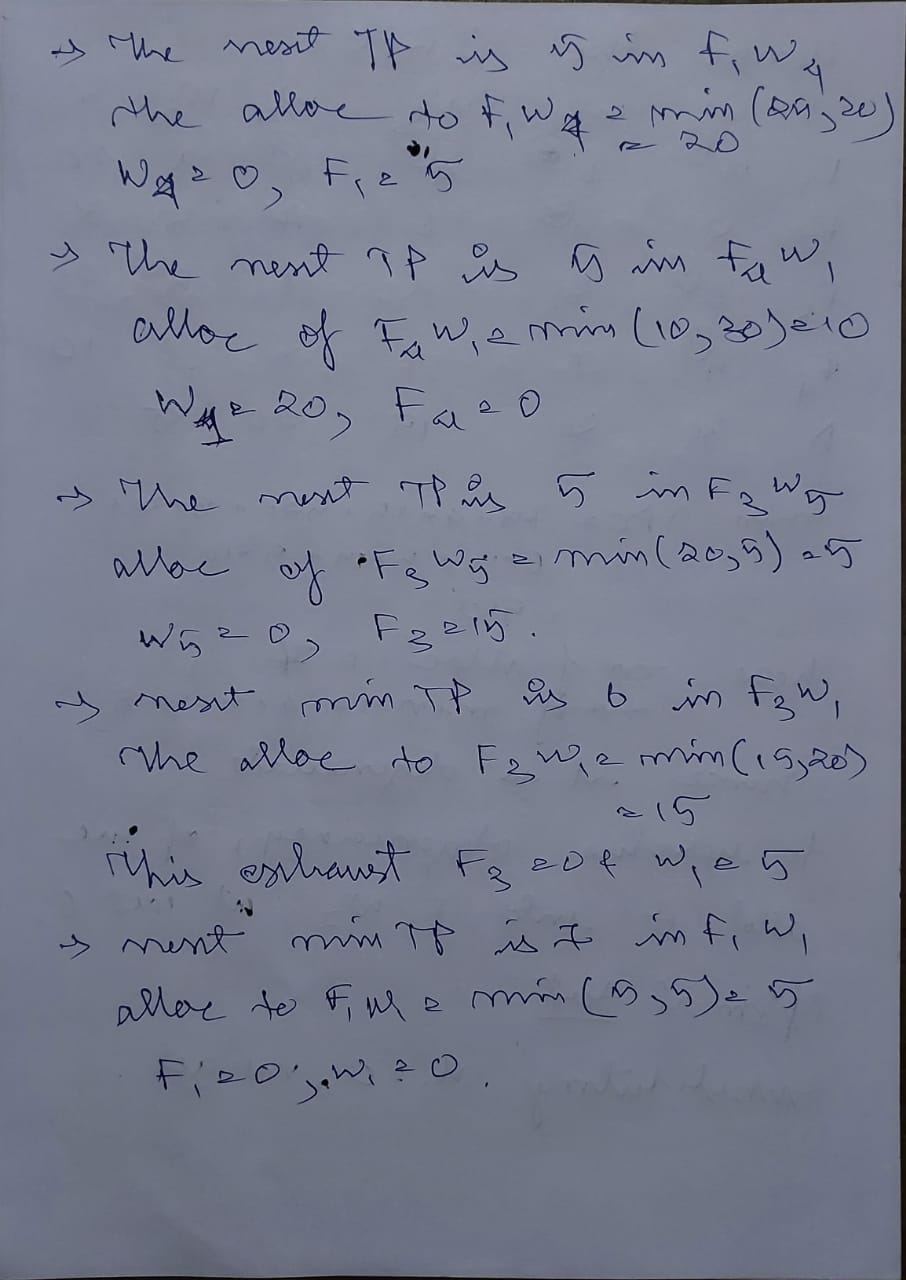
\includegraphics[width=\paperwidth, height=\paperheight]{Page21}
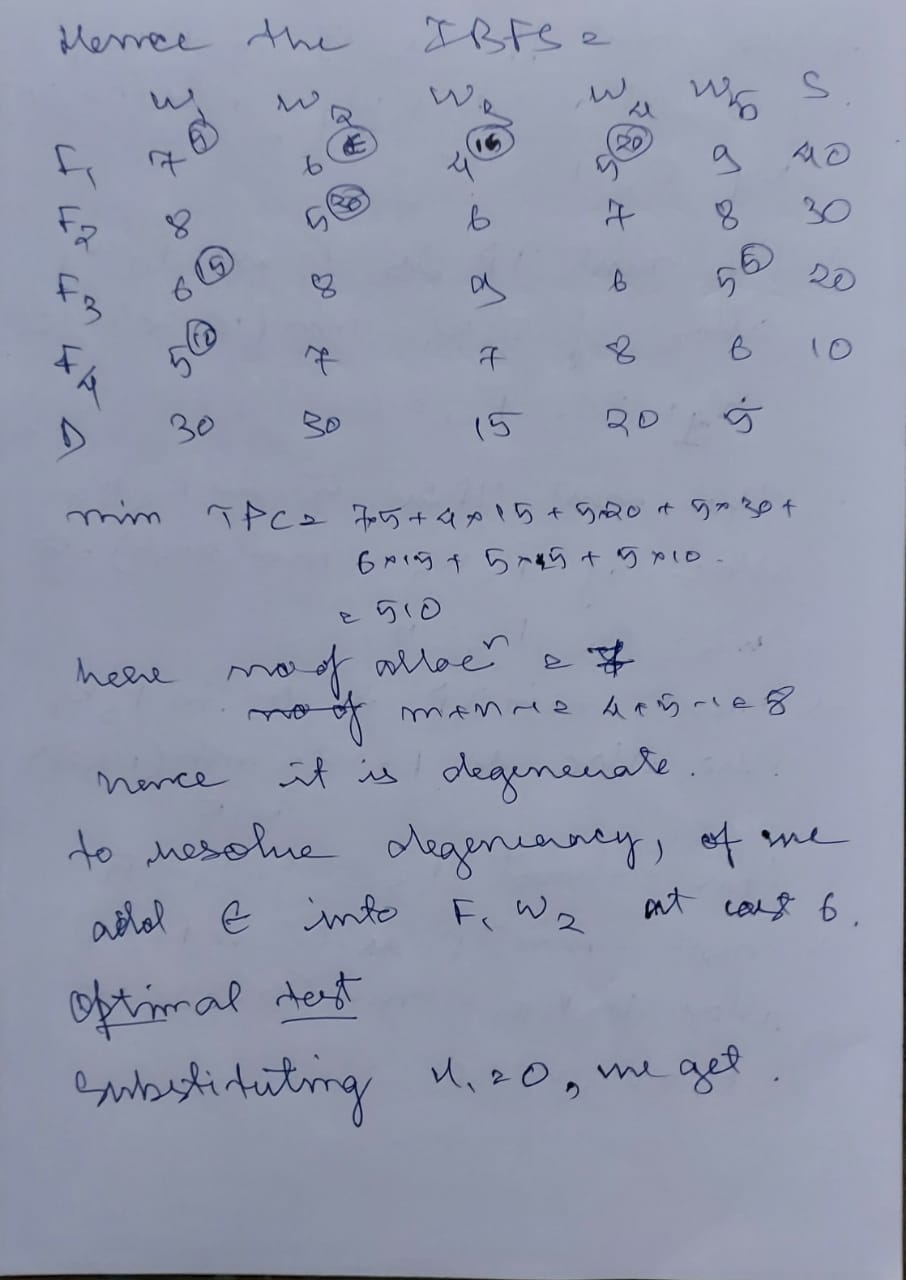
\includegraphics[width=\paperwidth, height=\paperheight]{Page22}
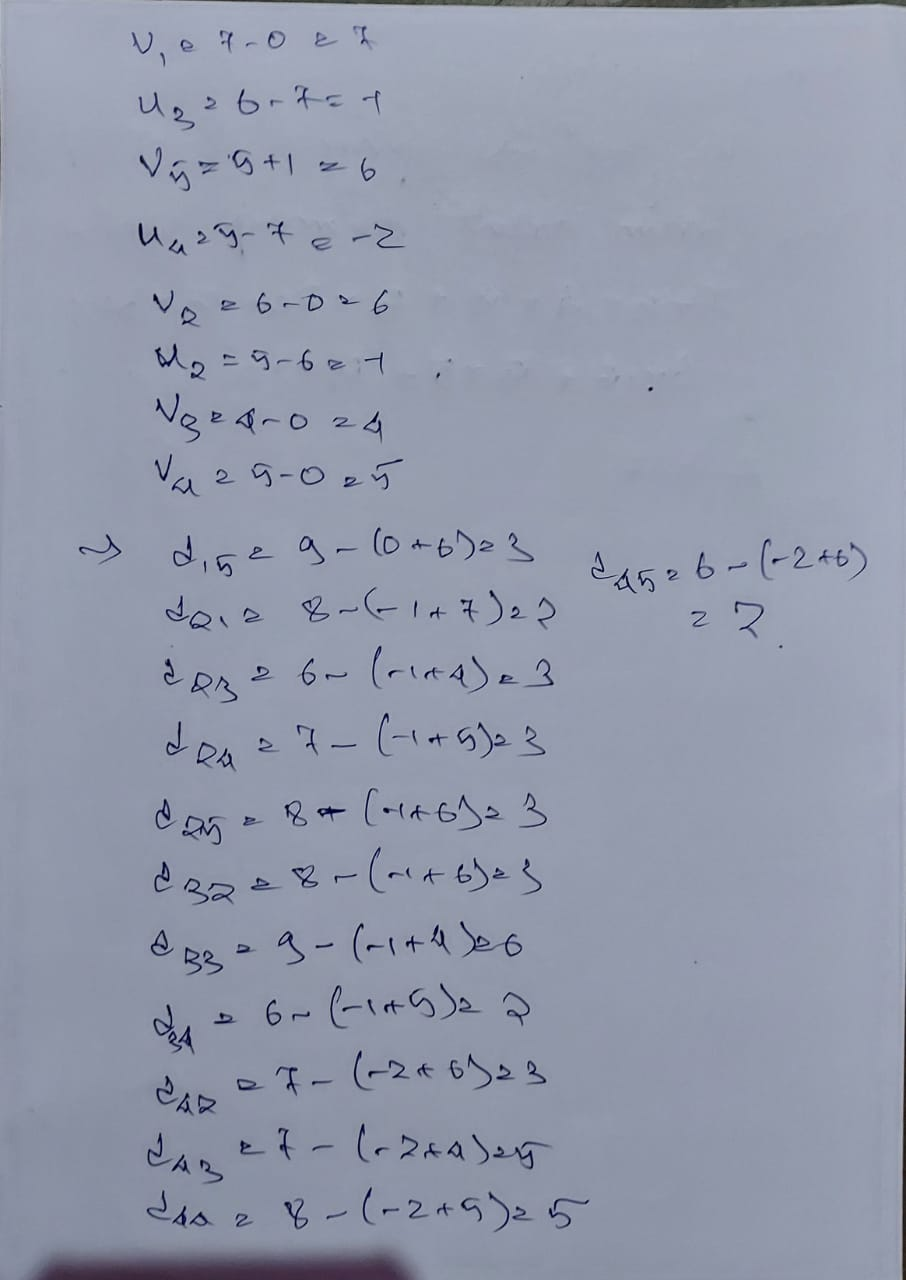
\includegraphics[width=\paperwidth, height=\paperheight]{Page23}
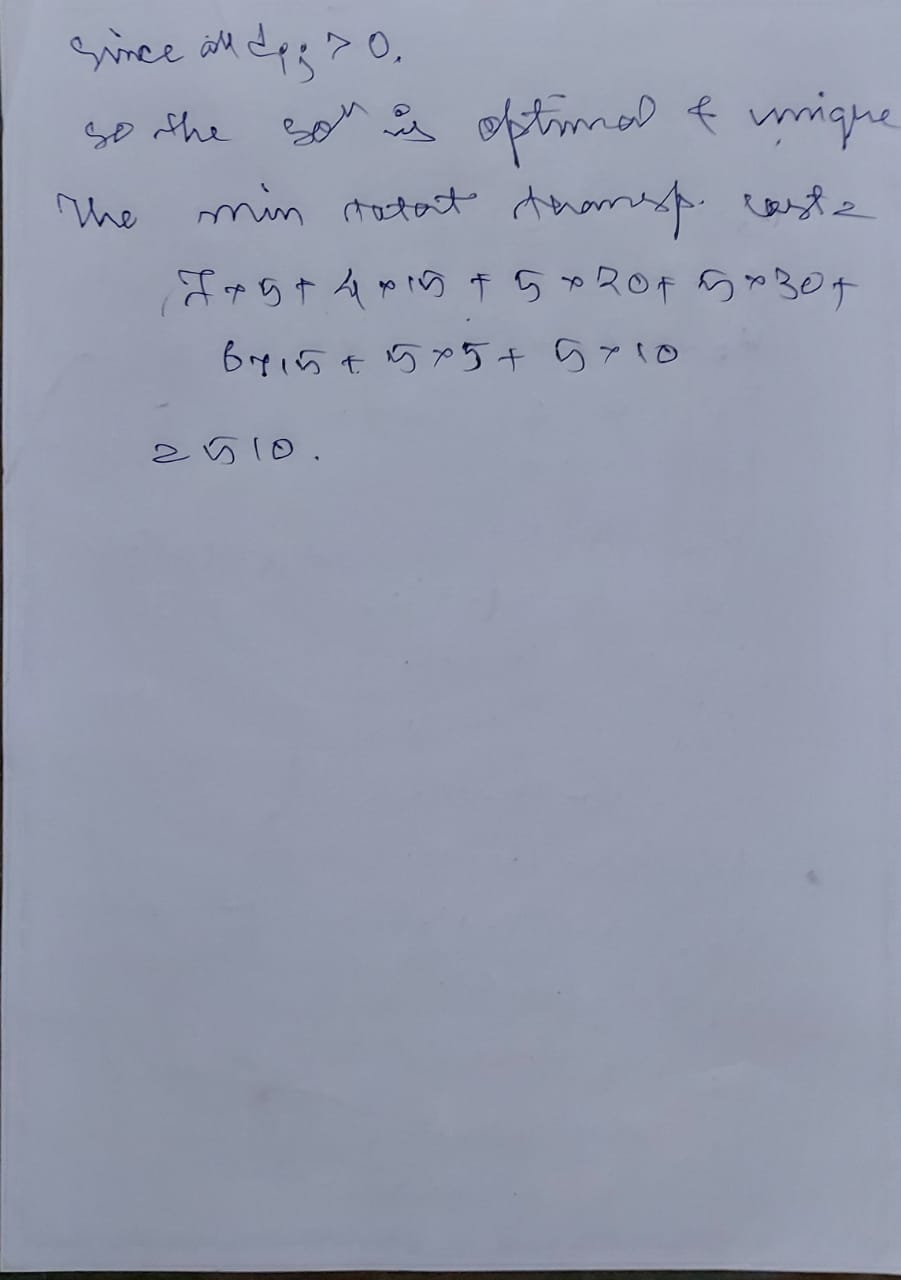
\includegraphics[width=\paperwidth, height=\paperheight]{Page24}
\begin{lstlisting}

	Python Code:
	
	import numpy as np
	from collections import Counter
	import math
	
	def check_loop(p, row, column):
		p[row, column] = -1
		flag = 1
		while flag != 0:
			flag = 0
			if p.size != 0:
				row = np.count_nonzero(p, axis=1)
				f = 0
				for index in range(len(row)):
					if row[index] < 2:
						flag = 1
						p = np.delete(p, (index - f), axis=0)
						f += 1
			if p.size != 0:
				e = 0
				col = np.count_nonzero(p, axis=0)
				for index in range(len(col)):
					if col[index] < 2:
						flag = 1
						p = np.delete(p, (index - e), axis=1)
						e += 1
		if p.size != 0:
			return 0
		else:
			return 1
	
	def max_allocation_row(non_zero_list):
		max_values = np.zeros(len(non_zero_list))
		for val in non_zero_list:
			max_values[val[0]] += 1.0
		return np.where(max_values == np.amax(max_values))
	
	
	def modi(c_modi, a_modi, m_modi, n_modi):
		iteration_count = 1
		while True:
		print()
		print("Iteration - ", iteration_count)
		print("Start AL \n", a_modi)
		u = np.array([np.nan] * m_modi)
		v = np.array([np.nan] * n_modi)
		p = np.zeros((m_modi, n_modi))
		_x, _y = np.where(a_modi > 0)
		nonzero = list(zip(_x, _y))
		_x1, _y1 = np.where(a_modi == -1)
		if -1 in a_modi:
			nz_a = np.where(a_modi == -1)
			nonzero.append((min(nz_a[0]), min(nz_a[1])))
		f = max_allocation_row(nonzero)
		u[f[0][0]] = 0
		for i, j in nonzero:
			if i == f[0][0]:
				v[j] = c_modi[i, j] - u[i]
		print("U = ", u)
		print("V = ", v)
		while any(np.isnan(u)) or any(np.isnan(v)):
			for i, j in nonzero:
				for j2 in range(0, len(v)):
					if j2 == j and not math.isnan(v[j]) 
						and math.isnan(u[i]):
						u[i] = c_modi[i, j] - v[j]
			for i, j in nonzero:
				for j2 in range(0, len(u)):
					if j2 == i and not math.isnan(u[i]) 
						and math.isnan(v[j]):
						v[j] = c_modi[i, j] - u[i]
			print("U = ", u)
			print("V = ", v)
			
		# Finding P-matrix
		for i in range(m_modi):
			for j in range(n_modi):
				if not nonzero.__contains__((i, j)):
					p[i, j] = c_modi[i, j] - u[i] - v[j]
		print("P-matrix")
		print(p)
		# Stop condition
		small_val = np.min(p)
		if small_val >= 0:
			break
		i, j = np.argwhere(p == small_val)[0]
		start = (i, j)
		print("Start : ", start)
		# Finding cycle elements
		t = np.copy(a_modi)
		t[start] = 1
		while True:
			_xs, _ys = np.nonzero(t)
			xcount, ycount = Counter(_xs), Counter(_ys)
			for x, count in xcount.items():
				if count <= 1:
					t[x, :] = 0
			for y, count in ycount.items():
				if count <= 1:
					t[:, y] = 0
			if all(x > 1 for x in xcount.values()) and 
				all(y > 1 for y in ycount.values()):
				break
		
		# Finding cycle chain order
		def dist(x1, y1, x2, y2):
			if x1 == x2 or y1 == y2:
				return abs(x1 - x2) + abs(y1 - y2)
			else:
				return np.inf
				
		fringe = set(tuple(p) for p in np.argwhere(t != 0))
		alloc_modi = fringe
		size = len(fringe)
		path = [start]
		while len(path) < size:
			last = path[-1]
			if last in fringe:
				fringe.remove(last)
			next_val = min(fringe, key=lambda xy: dist(last[0], 
				last[1], xy[0], xy[1]))
			path.append(next_val)
			
		# Improving solution on cycle elements
		neg = path[1::2]
		pos = path[::2]
		print("Negative Value:", neg)
		print("Positive Value:", pos)
		ql = []
		for row in neg:
			ql.append(a_modi[row[0], row[1]])
		q = int(min(ql))
		for row in neg:
			if a_modi[row[0], row[1]] == -1:
				a_modi[row[0], row[1]] = 0 - q
			else:
				a_modi[row[0], row[1]] -= q
		for row in pos:
			if a_modi[row[0], row[1]] == -1:
				a_modi[row[0], row[1]] = 0 + q
			else:
				a_modi[row[0], row[1]] += q
		x_al = np.nonzero(a_modi)[0]
		y_al = np.nonzero(a_modi)[1]
		for i in range(len(x_al)):
			alloc_modi.add((x_al[i], y_al[i]))
		print("Mid Allocation Table : \n", a_modi)
		
		_x2, _y2 = np.where(a_modi > 0)
		# alloc_modi = list(zip(_x2, _y2))
		no_alloc_modi = np.count_nonzero(a_modi)
		unalloc_modi = []
		for i1 in range(m_modi):
			for j1 in range(n_modi):
				if not (i1, j1) in alloc_modi:
					unalloc_modi.append((i1, j1))
		print(a_modi)
		no_loop_modi = []
		if no_alloc_modi == m_modi + n_modi - 1:
			print("Non Degeneracy")
		else:
			print("Degeneracy")
			print("Values of epsilon is -1")
			for i1 in unalloc_modi:
				if check_loop(a_modi.copy(), i1[0], i1[1]) == 1:
					no_loop_modi.append(i1)
			min_epi_list = []
			for i1 in no_loop_modi:
				min_epi_list.append(c_modi[i1[0], i1[1]])
			min_epi = min(min_epi_list)
			ind = min_epi_list.index(min_epi)
			loc = no_loop_modi[ind]
			a_modi[loc[0], loc[1]] = -1
			print("END AL : \n", a_modi)
			print()
		iteration_count += 1
	return a_modi


	def nwcr(cm_nwcr, m_nwcr, n_nwcr, s_nwcr, d_nwcr):
		c_nwcr = cm_nwcr.copy()
		a = np.zeros(c_nwcr.shape)
		total_cost_nwcr = 0
		no_alloc_nwcr = 0
		alloc_nwcr = []
		i = 0
		j = 0
		while (i < m_main) and (j < n_main):
			x = min(s_nwcr[i], d_nwcr[j])
			s_nwcr[i] = s_nwcr[i] - x
			d_nwcr[j] = d_nwcr[j] - x
			total_cost_nwcr = total_cost_nwcr + x * c_nwcr[i, j]
			no_alloc_nwcr += 1
			alloc_nwcr.append((i, j))
			a[i, j] = x
			if s_nwcr[i] < d_nwcr[j]:
				i = i + 1
			elif s_nwcr[i] > d_nwcr[j]:
				j = j + 1
			else:
				i = i + 1
				j = j + 1
		print("Total Cost: ", total_cost_nwcr)
		unalloc_nwcr = []
		for i1 in range(m_main):
			for j1 in range(n_main):
				if not (i1, j1) in alloc_nwcr:
					unalloc_nwcr.append((i1, j1))
		print("Allocated Positions: ", alloc_nwcr)
		print("Unallocated Positions: ", unalloc_nwcr)
		print("Allocation Matrix: ")
		print(a)
		no_loop_nwcr = []
		if no_alloc_nwcr == m_nwcr + n_nwcr - 1:
			print("Non Degeneracy")
		else:
			print("Degeneracy")
			print("Values of epsilon is -1")
			for i1 in unalloc_nwcr:
				if check_loop(a.copy(), i1[0], i1[1]) == 1:
					no_loop_nwcr.append(i1)
			min_epi_list = []
			for i1 in no_loop_nwcr:
				min_epi_list.append(cm_nwcr[i1[0], i1[1]])
			min_epi = min(min_epi_list)
			ind = min_epi_list.index(min_epi)
			loc = no_loop_nwcr[ind]
			a[loc[0], loc[1]] = -1
			print("Allocation Matrix After Converting Degeneracy 
				to Non-Degeneracy is : ")
			print(a)
		optl = modi(cm_nwcr.copy(), a.copy(), m_nwcr, n_nwcr, )
		print('optimised Allocation Matrix: ')
		print(optl)
		for row in range(0, m_nwcr):
			for column in range(0, n_nwcr):
				if optl[row][column] < 0:
					optl[row][column] = 0
		print("Total Optimal Cost = ", np.sum(optl * cm_nwcr))

		
	def lcm(cm_lcm, m_lcm, n_lcm, s_lcm, d_lcm):
		c_lcm = cm_lcm.copy()
		total_cost_lcm = 0
		no_alloc_lcm = 0
		alloc_lcm = []
		a = np.zeros(c_lcm.shape)
		min_cost = np.amin(c_lcm)
		while min_cost != np.inf:
			indexes = np.where(c_lcm == min_cost)
			i = indexes[0][0]
			j = indexes[1][0]
			x = min(s[i], d_lcm[j])
			s_lcm[i] -= x
			d_lcm[j] -= x
			total_cost_lcm += (x * c_lcm[i, j])
			no_alloc_lcm += 1
			a[i, j] = x
			alloc.append((i, j))
			if s_lcm[i] < d_lcm[j]:
				x = 0
				while x < n_lcm:
					c_lcm[i, x] = np.inf
					x += 1
			elif s_lcm[i] > d_lcm[j]:
				y = 0
				while y < m_lcm:
					c_lcm[y, j] = np.inf
					y += 1
			else:
				x = 0
				while x < n_lcm:
					c_lcm[i, x] = np.inf
					x += 1
				y = 0
				while y < m_lcm:
					c_lcm[y, j] = np.inf
					y += 1
			min_cost = np.amin(c_lcm)
		print("Total Cost: ", total_cost_lcm)
		unalloc = []
		for i in range(m_lcm):
			for j in range(n_lcm):
				if not (i, j) in alloc:
					unalloc.append((i, j))
		print("List of Allocated Positions: ", alloc)
		print("List of Unallocated Positions: ", unalloc)
		print("Allocation Matrix: ")
		print(a)
		no_loop_lcm = []
		if no_alloc_lcm == m_lcm + n_lcm - 1:
			print("Non Degeneracy")
		else:
			print("Degeneracy")
			for i in unalloc:
				g = check_loop(a.copy(), i[0], i[1])
				if g == 1:
					no_loop_lcm.append(i)
				min_epi_list = []
			for i in no_loop_lcm:
				min_epi_list.append(cm[i[0], i[1]])
			min_epi = min(min_epi_list)
			ind = min_epi_list.index(min_epi)
			loc = no_loop_lcm[ind]
			a[loc[0], loc[1]] = -1
			print("Allocation Matrix After Converting 
				Degeneracy to Non-Degeneracy is : ")
			print(a)
		optl = modi(cm_lcm.copy(), a.copy(), m_lcm, n_lcm, )
		print('optimised Allocation Matrix: ')
		print(optl)
		for row in range(0, m_lcm):
			for column in range(0, n_lcm):
				if optl[row][column] < 0:
					optl[row][column] = 0
		print("Total Optimal Cost = ", np.sum(optl * cm_lcm))

\end{lstlisting}
\pagebreak
\begin{lstlisting}    
		
	if __name__ == '__main__':
		cm_main = np.array([[7.0, 6, 4, 5, 9],
			[8, 5, 6, 7, 8],
			[6, 8, 9, 6, 5],
			[5, 7, 7, 8, 6]])
		s_main = np.array([40.0, 30, 20, 10])
		d_main = np.array([30.0, 30, 15, 20, 5])
		c_main = cm_main.copy()
		print("The Cost Matrix is: ")
		print(c_main)
		print("The Supply is: ", s_main)
		print("The Demand is: ", d_main)
		m_main, n_main = c_main.shape
		print("No of Rows & No of Columns: (", m_main, ", ", n_main, ")")
		total_demand = np.sum(d_main)
		total_supply = np.sum(s_main)
		if total_demand == total_supply:
			print("It is a Balanced Transportation Problem")
		else:
			print("It is an UnBalanced Transportation Problem")
			if total_demand > total_supply:
				new = np.array(np.zeros(n_main))
				c_main = np.row_stack((c_main, new))
				s_main = np.append(s, total_demand - total_supply)
				m_main = m_main + 1
			else:
				new = np.array(np.zeros(m_main))
				c_main = np.column_stack((c_main, new))
				d = np.append(d, total_supply - total_demand)
				n_main = n_main + 1
			print("The New Balanced Cost Matrix is: ")
			print(c_main)
			print("The Supply is: ", s_main)
			print("The Demand is: ", d_main)
		print("Northwest corner method")
		nwcr(c_main.copy(), m_main, n_main, s_main.copy(), d_main.copy())
		print()
		print("Least Cost Method")
		lcm(c_main.copy(), m_main, n_main, s_main.copy(), d_main.copy())
		print()

\end{lstlisting}
\pagebreak
\begin{lstlisting}

	Output:

\end{lstlisting}

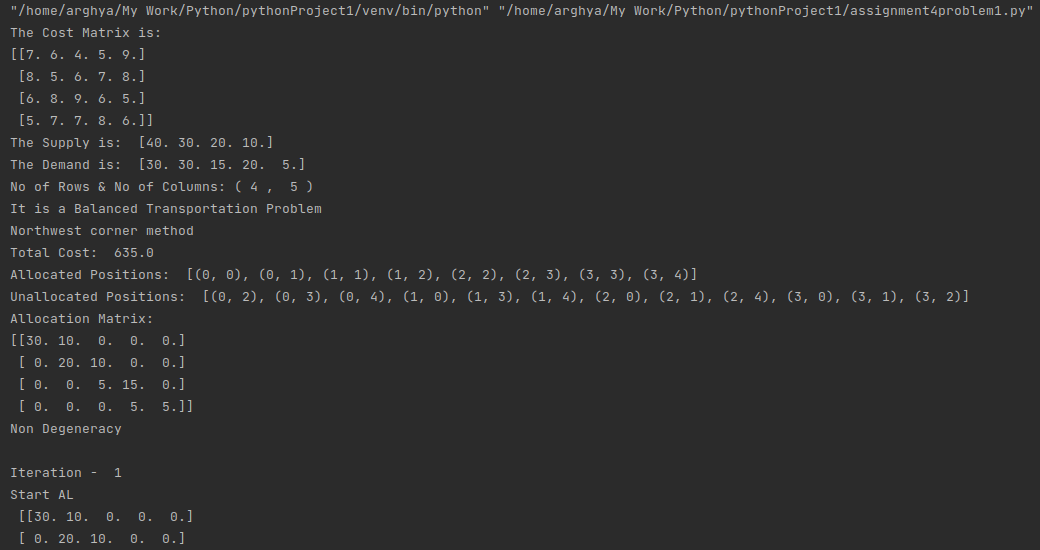
\includegraphics[width=550pt]{Output1}

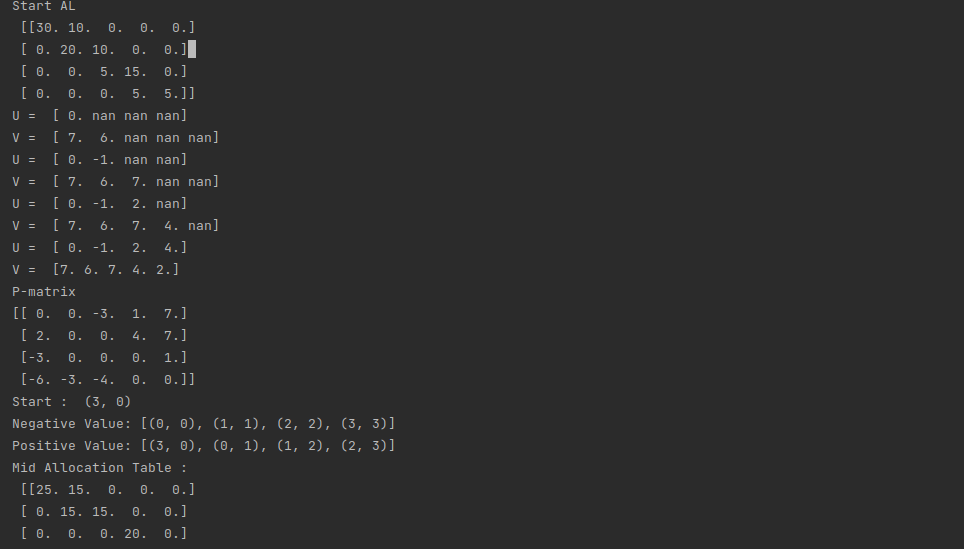
\includegraphics[width=550pt]{Output2}


\includegraphics[width=550pt]{Output3}

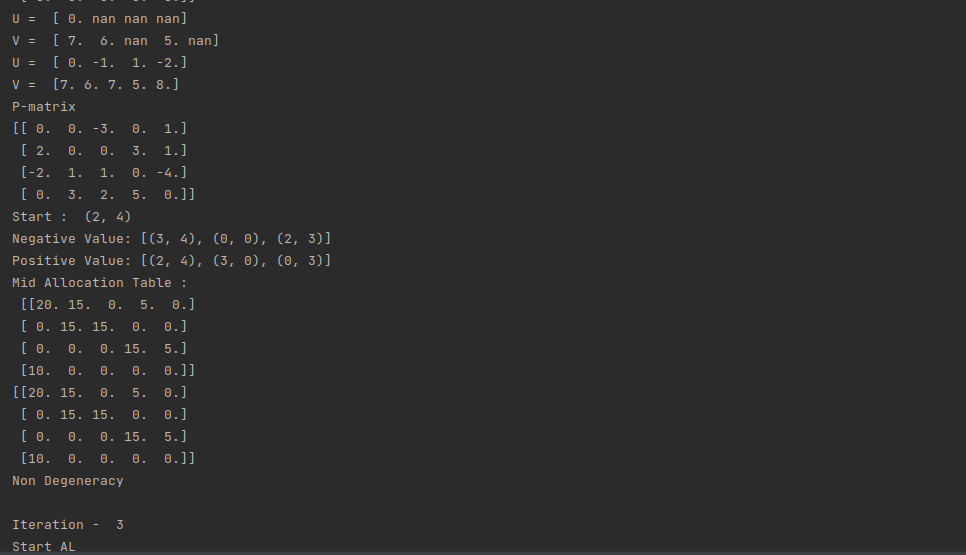
\includegraphics[width=550pt]{Output4}

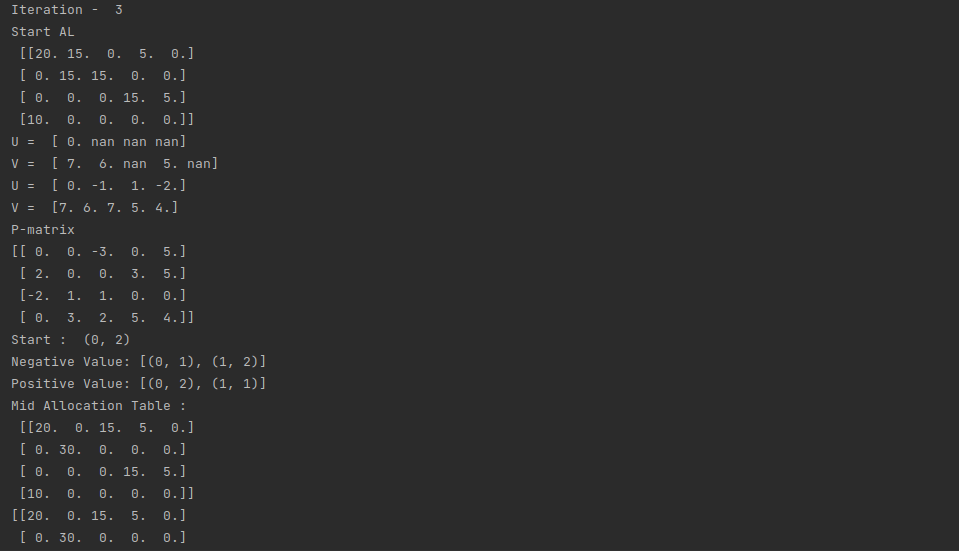
\includegraphics[width=550pt]{Output5}

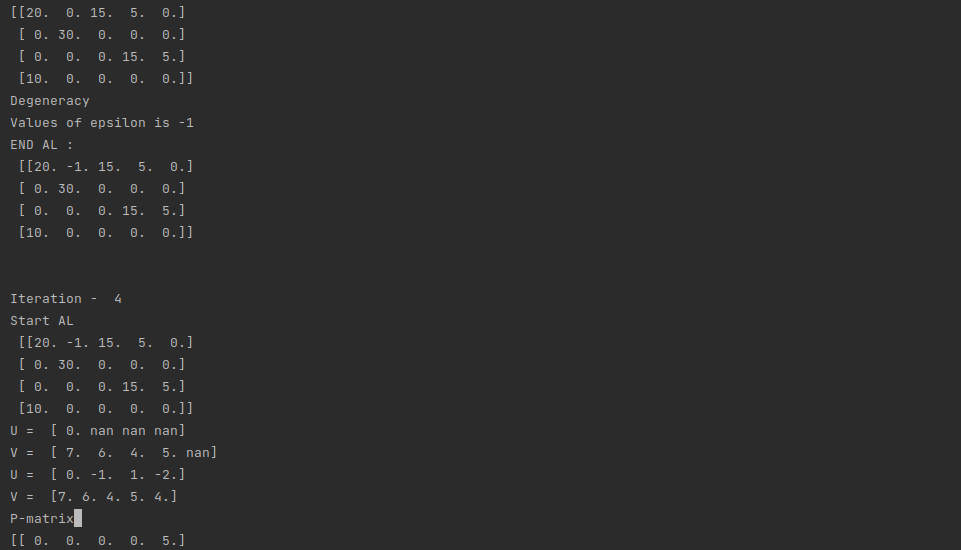
\includegraphics[width=550pt]{Output6}

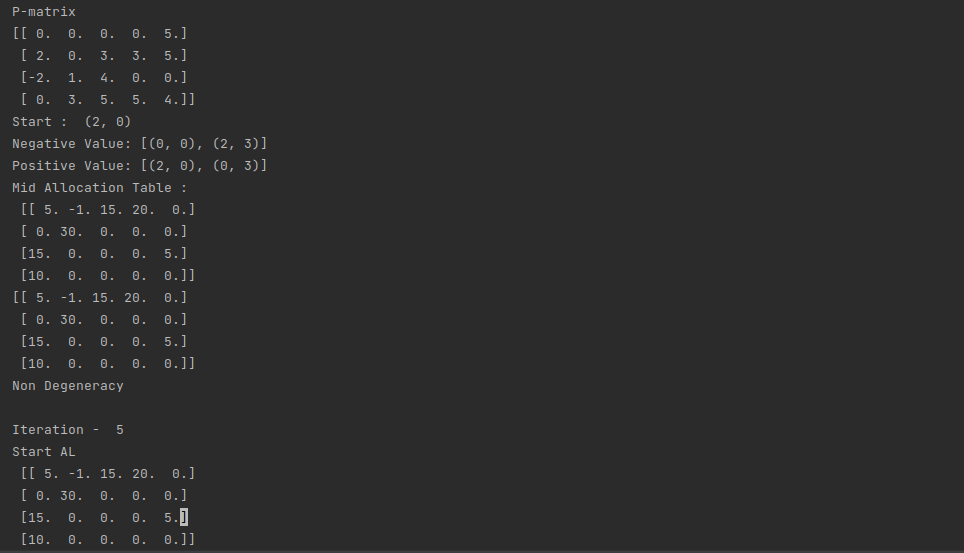
\includegraphics[width=550pt]{Output7}

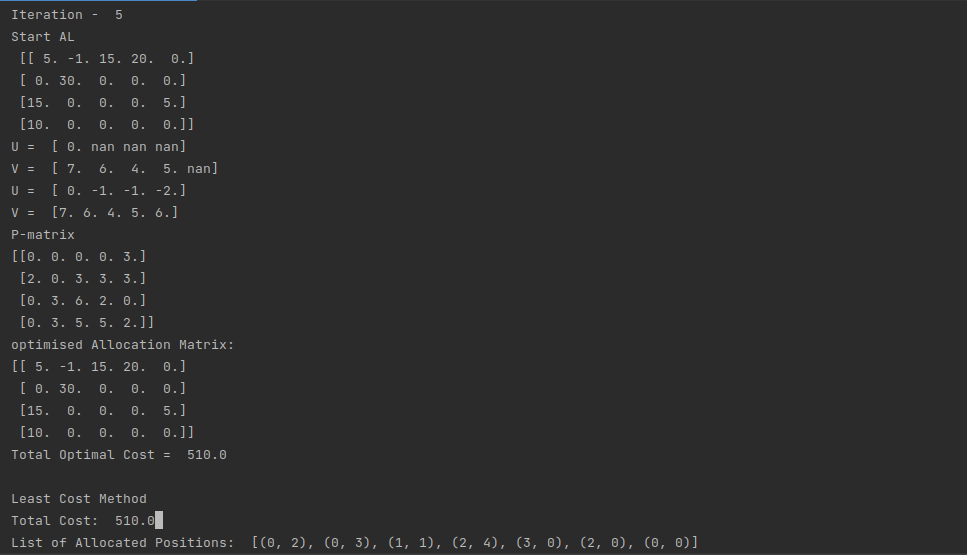
\includegraphics[width=550pt]{Output8}

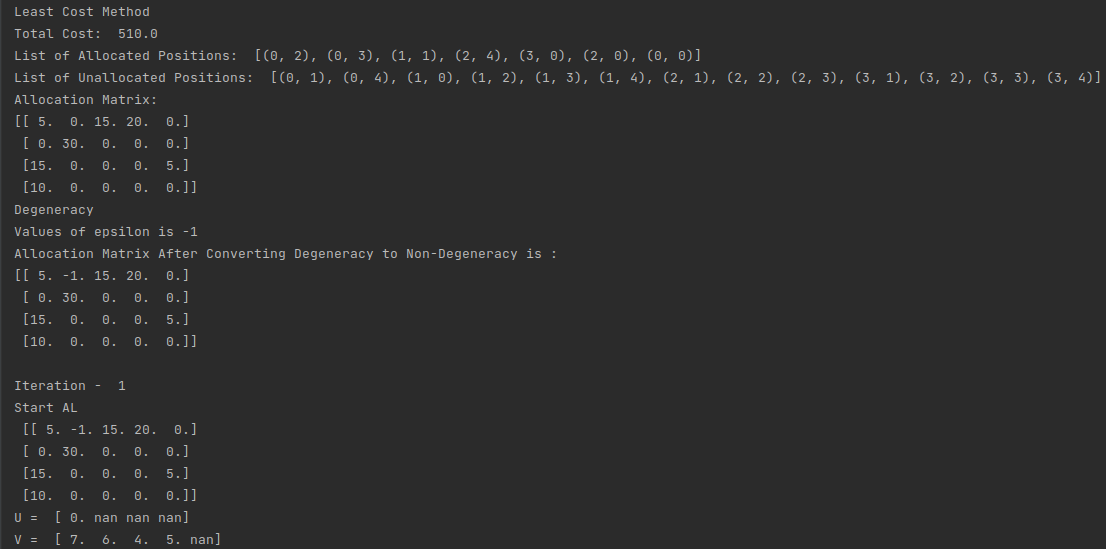
\includegraphics[width=550pt]{Output9}

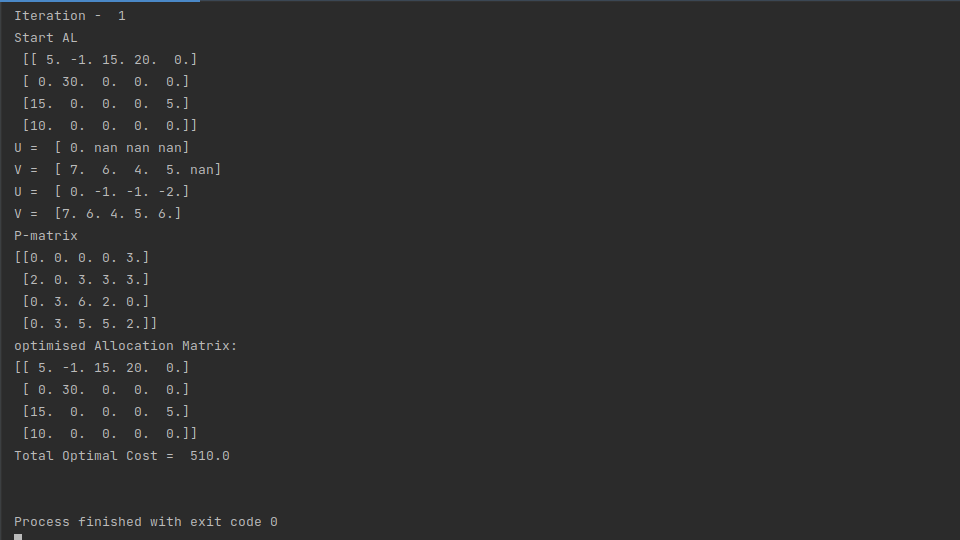
\includegraphics[width=550pt]{Output10}

\pagebreak
\end{document}
